% =============================================================================
% Parte 1 — Conoce el x500: del dron real a tu primer nodo
% Vespo UAV
%
% La parte visual, para la primera sesión. La Parte 2 (main.tex) es la
% referencia técnica para cuando programen.
%
% Compilar:  latexmk -pdf parte1.tex
% Fotos de PX4 (CC BY 4.0) en img/px4docs, renders propios en img/render.
% =============================================================================
\documentclass[aspectratio=169,10pt]{beamer}
% =============================================================================
% PX4 + ROS 2 con px4_examples — Vespo UAV
%
% Compilar:  latexmk -pdf main.tex      (o pdflatex dos veces, por los índices)
% Necesita:  texlive-latex-extra texlive-lang-spanish texlive-pictures
%            texlive-fonts-recommended
%
% Cada sección vive en secciones/NN_nombre.tex. Todo lo que se cita del código
% sale de src/px4_examples/src/*.cpp.
% =============================================================================
% (el \documentclass va en cada presentación)

\usepackage[utf8]{inputenc}
\usepackage[T1]{fontenc}
\usepackage[spanish,es-nodecimaldot,es-noshorthands]{babel}
\usepackage{amsmath,amssymb}
\usepackage{booktabs}
\usepackage{graphicx}
\usepackage{xcolor}
\usepackage{listings}
\usepackage[most]{tcolorbox}
\usepackage{tikz}
\usetikzlibrary{arrows.meta,positioning,shapes.geometric,shapes.misc,calc,fit,backgrounds,decorations.pathreplacing}
\usepackage{multicol}
\usepackage{pifont}
% Lo que imprime vespo en la terminal
\DeclareUnicodeCharacter{2714}{\ding{51}}
\DeclareUnicodeCharacter{2718}{\ding{55}}
\DeclareUnicodeCharacter{2500}{\textendash}

\graphicspath{{img/}{img/px4docs/}{img/render/}{../../../x500_retos/docs/img/}}

% --- Tema: el de la intro a ROS2 ---------------------------------------------
\usetheme{default}
\useoutertheme{infolines}
\setbeamertemplate{headline}{}
\setbeamercolor{author in head/foot}{fg=black,bg=white}
\setbeamercolor{title in head/foot}{fg=blue!70!black,bg=white}
\setbeamercolor{date in head/foot}{fg=black,bg=white}
\setbeamercolor{section in toc}{fg=blue!70!black}
\setbeamertemplate{section in toc}[circle]
\setbeamercolor{frametitle}{fg=black,bg=white}
\setbeamerfont{frametitle}{size=\Large}
\setbeamertemplate{frametitle}{%
  \vskip0.4em
  \begin{beamercolorbox}[wd=\paperwidth,leftskip=0.3em,rightskip=0.3em]{frametitle}%
    \usebeamerfont{frametitle}\insertframetitle\hfill
    \raisebox{-0.45em}{
\includegraphics[height=1.6em]{vespo_logo}}%
  \end{beamercolorbox}}
\setbeamertemplate{caption}[numbered]
\setbeamertemplate{itemize items}[circle]
\setbeamercolor{itemize item}{fg=blue!70!black}
\setbeamercolor{enumerate item}{fg=blue!70!black}

% --- Colores y cajas -------------------------------------------------------------
\definecolor{azul}{RGB}{40,80,180}
\definecolor{azulclaro}{RGB}{232,238,252}
\definecolor{verde}{RGB}{0,128,0}
\definecolor{verdeclaro}{RGB}{236,250,236}
\definecolor{rojo}{RGB}{190,30,30}
\definecolor{naranja}{RGB}{230,120,10}
\definecolor{gris}{RGB}{110,110,110}

% Idea clave: caja azul redondeada con sombra.
\newtcolorbox{idea}[1][]{enhanced,colback=azulclaro,colframe=azul!40,arc=2mm,
  boxrule=0.4pt,drop shadow,left=1.5mm,right=1.5mm,top=1mm,bottom=1mm,#1}
% Ojo: lo que suele salir mal.
\newtcolorbox{ojo}[1][]{enhanced,colback=red!5,colframe=rojo!60,arc=2mm,boxrule=0.4pt,
  drop shadow,left=1.5mm,right=1.5mm,top=1mm,bottom=1mm,
  title={\small\bfseries Ojo},fonttitle=\small,coltitle=white,colbacktitle=rojo!80,#1}
% Salida de terminal: barra verde con el comando.
\newtcolorbox{terminal}[1]{enhanced,colback=verdeclaro,colframe=verde,arc=1mm,boxrule=0.6pt,
  title={\ttfamily\small #1},fonttitle=\ttfamily\small,coltitle=white,colbacktitle=verde,
  left=1mm,right=1mm,top=0.5mm,bottom=0.5mm,fontupper=\ttfamily\scriptsize}

% --- Código ----------------------------------------------------------------------
\renewcommand{\lstlistingname}{Código}
\lstset{
  basicstyle=\ttfamily\scriptsize,
  keywordstyle=\color{azul}\bfseries,
  commentstyle=\color{gris}\itshape,
  stringstyle=\color{verde},
  frame=single, rulecolor=\color{black},
  breaklines=true, columns=fullflexible, keepspaces=true,
  showstringspaces=false, captionpos=b, tabsize=2,
  xleftmargin=2pt, xrightmargin=2pt, aboveskip=4pt, belowskip=2pt,
  literate=
    {á}{{\'a}}1 {é}{{\'e}}1 {í}{{\'i}}1 {ó}{{\'o}}1 {ú}{{\'u}}1
    {Á}{{\'A}}1 {É}{{\'E}}1 {Í}{{\'I}}1 {Ó}{{\'O}}1 {Ú}{{\'U}}1
    {ñ}{{\~n}}1 {Ñ}{{\~N}}1 {ü}{{\"u}}1 {¿}{{?`}}1 {¡}{{!`}}1
    {°}{{$^\circ$}}1 {²}{{$^2$}}1 {·}{{$\cdot$}}1
    {→}{{$\rightarrow$}}2 {←}{{$\leftarrow$}}2 {≈}{{$\approx$}}1
    {▲}{{$\blacktriangle$}}1 {►}{{$\blacktriangleright$}}1 {│}{{|}}1 {─}{{-}}1
    {┌}{{+}}1 {┐}{{+}}1 {└}{{+}}1 {┘}{{+}}1 {├}{{+}}1 {┤}{{+}}1 {┼}{{+}}1
}
\lstdefinestyle{cpp}{language=C++,morekeywords={override,nullptr,constexpr,auto}}
\lstdefinestyle{bash}{language=bash,morekeywords={ros2,vespo,colcon}}
\lstdefinelanguage{yaml}{morecomment=[l]\#,morestring=[b]"}

% --- Atajos ---------------------------------------------------------------------
\newcommand{\cmd}[1]{\texttt{#1}}
\newcommand{\ok}{{\color{verde}\checkmark}}
\newcommand{\mal}{{\color{rojo}$\times$}}

% Al empezar cada sección: el contenido con la sección actual resaltada.
\AtBeginSection[]{%
  \begin{frame}{Contenido}
    \begin{multicols}{2}\scriptsize
      \tableofcontents[currentsection]
    \end{multicols}
  \end{frame}}

% Láminas que se arman paso a paso: en TikZ, "visible on=<3->" muestra un
% nodo desde el paso 3 y "alt=<2>{fill=...}{fill=...}" lo resalta en el paso 2.
\tikzset{
  invisible/.style={opacity=0,text opacity=0},
  visible on/.style={alt={#1{}{invisible}}},
  alt/.code args={<#1>#2#3}{\alt<#1>{\pgfkeysalso{#2}}{\pgfkeysalso{#3}}},
}
\newcommand{\credito}[1]{{\tiny\color{gris}#1}}

% El x500 recortado (tools/renders_x500.py + tools/recortar_iconos.py).
% \dronarriba{ancho}: visto desde arriba, la nariz hacia arriba de la imagen.
% Para girarlo a un yaw (0 = norte, positivo hacia el este) en TikZ: \node[rotate=-yaw].
\newcommand{\dronarriba}[1]{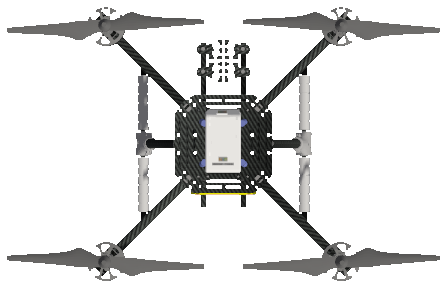
\includegraphics[width=#1]{x500_icono}}
\newcommand{\dronlado}[1]{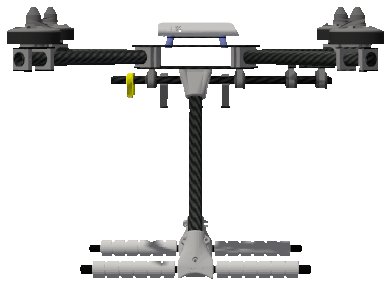
\includegraphics[width=#1]{x500_lado_icono}}


\title[Conoce el x500]{Conoce el x500}
\subtitle{Del dron real a tu primer nodo de ROS 2 (Parte 1)}
\author[Imad Cabrera]{Imad Jared Cabrera Trejo}
\institute[Vespo UAV]{Vespo UAV Drones Autónomos}
\date{11 de noviembre de 2026}

\begin{document}

\begin{frame}[plain]
  \begin{tikzpicture}[remember picture,overlay]
    \node at (current page.center) {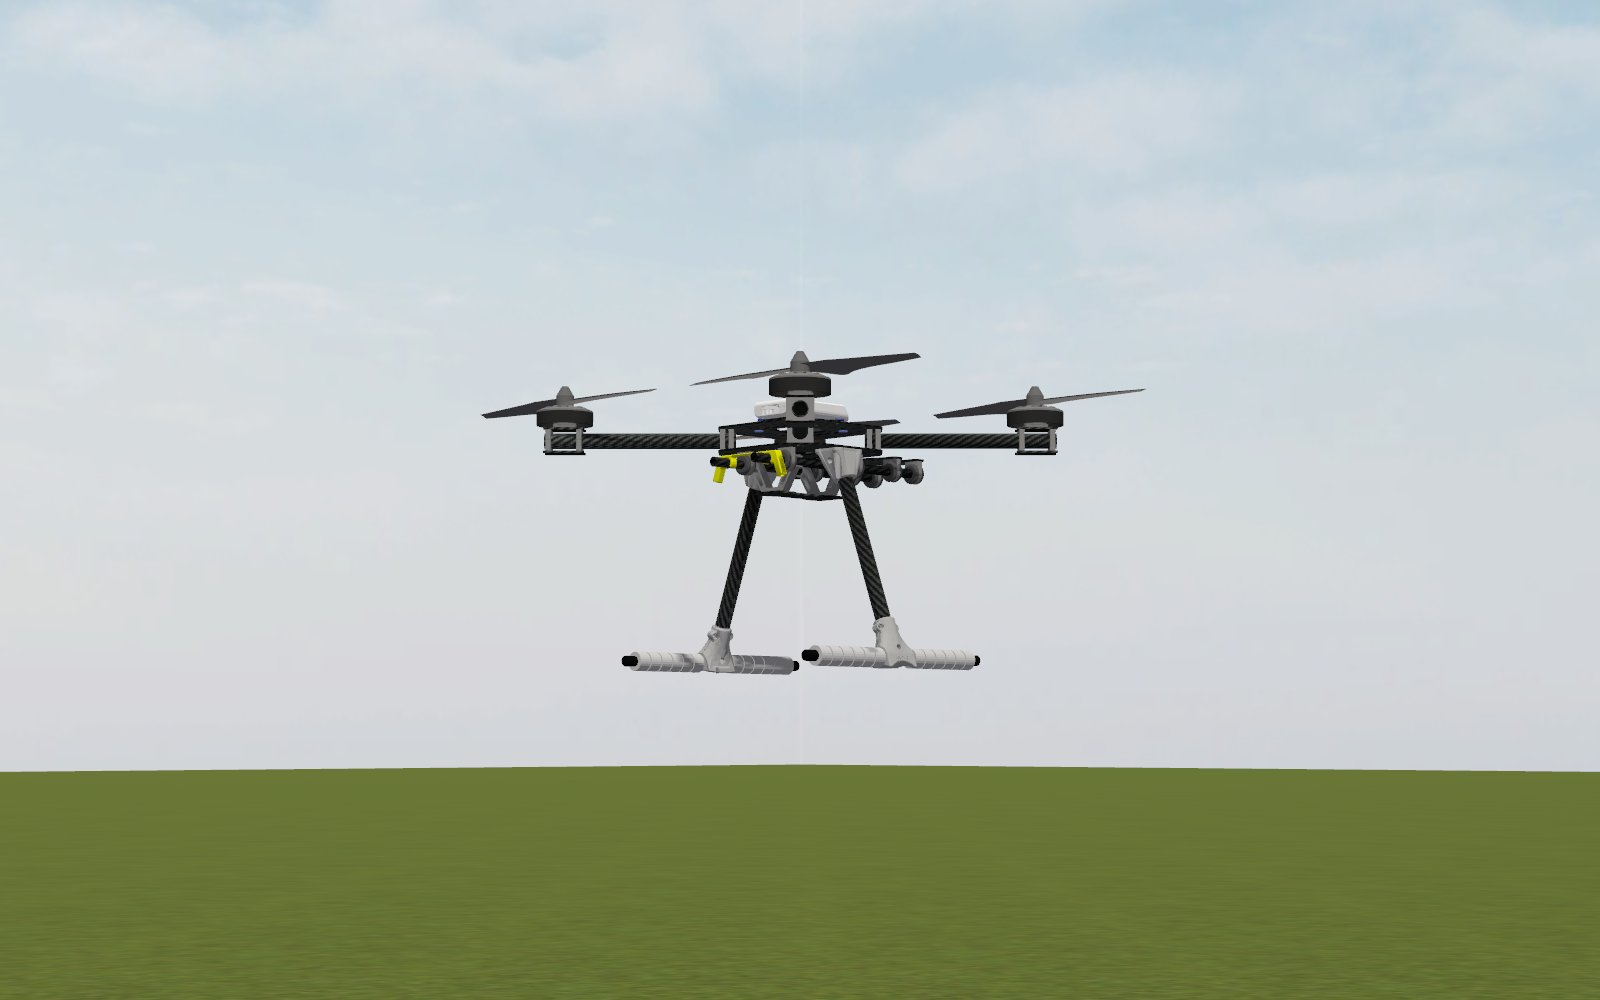
\includegraphics[width=\paperwidth]{x500_volando}};
    \fill[white,opacity=0.78] ([yshift=-1.6cm]current page.north west) rectangle ([yshift=-4.4cm]current page.north east);
    \node[font=\LARGE\bfseries] at ([yshift=-2.5cm]current page.north) {Conoce el x500};
    \node[font=\normalsize] at ([yshift=-3.3cm]current page.north) {Del dron real a tu primer nodo de ROS 2 (Parte 1)};
    \node[font=\scriptsize] at ([yshift=-3.9cm]current page.north) {Imad Jared Cabrera Trejo · Vespo UAV · 11 de noviembre de 2026};
    \node[anchor=south east] at ([xshift=-0.3cm,yshift=0.3cm]current page.south east) {
\includegraphics[height=1.1cm]{vespo_logo}};
  \end{tikzpicture}
\end{frame}

\begin{frame}{Hoy}
  \begin{columns}[c]
    \column{0.55\textwidth}
    \begin{enumerate}
      \item \textbf{El dron}: qué piezas tiene y qué hace cada una.
      \item \textbf{Su gemelo}: el mismo x500, en la simulación.
      \item \textbf{Quién hace qué}: tu programa, PX4, QGroundControl y Gazebo.
      \item \textbf{El viaje de un comando}: qué pasa desde que das Enter hasta que el dron sube.
      \item \textbf{Lo que vas a ver} en tu pantalla.
      \item \textbf{Tu primer vuelo}, paso a paso.
    \end{enumerate}
    \column{0.42\textwidth}
    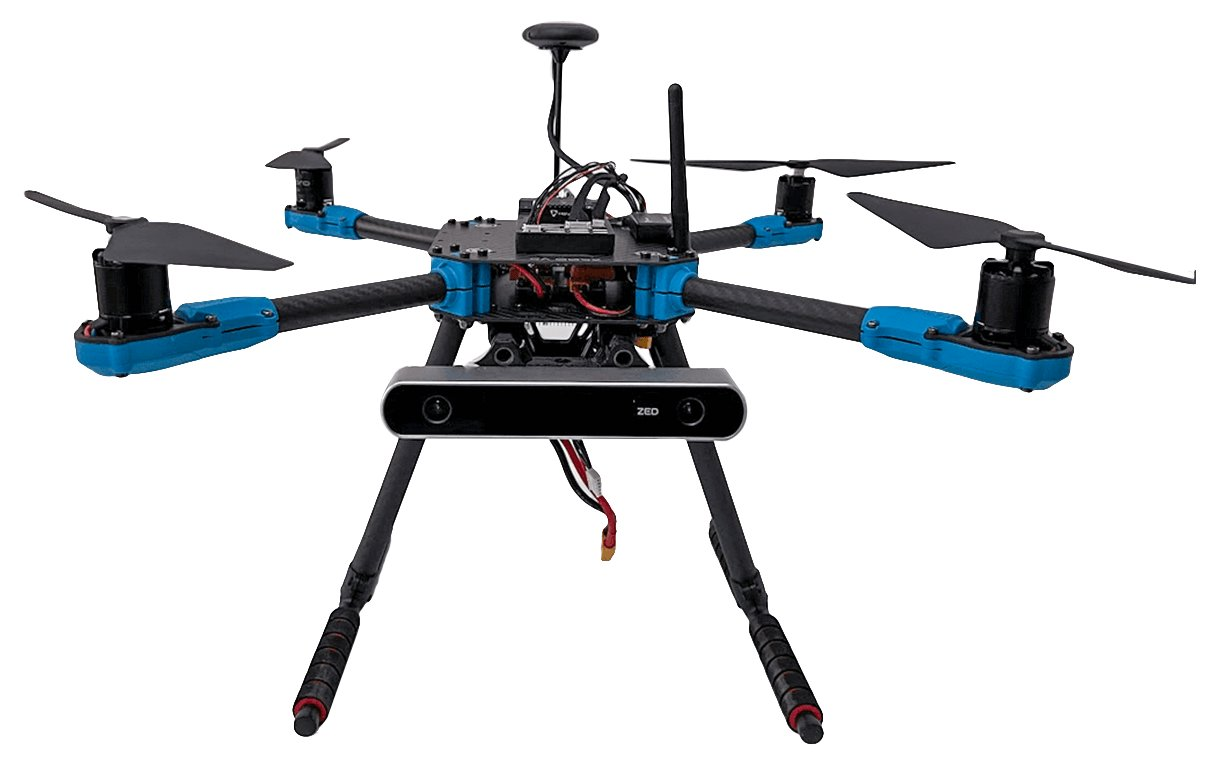
\includegraphics[width=\linewidth]{x500v2_armado}\\
    \credito{Foto: documentación de PX4 (CC BY 4.0)}
  \end{columns}
\end{frame}

% =============================================================================
\section{El dron}
% =============================================================================

\begin{frame}{Este es el x500}
  \begin{columns}[c]
    \column{0.55\textwidth}
    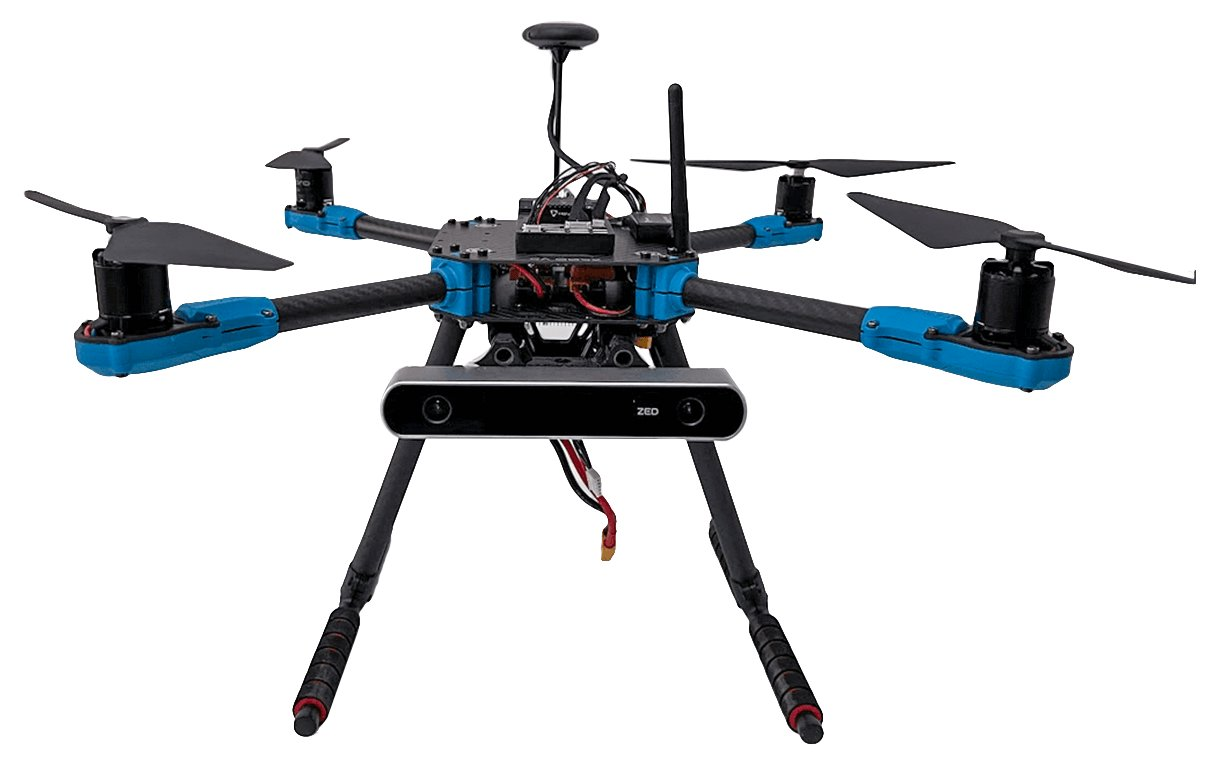
\includegraphics[width=\linewidth]{x500v2_armado}\\
    \credito{Holybro X500 V2. Foto: documentación de PX4 (CC BY 4.0)}
    \column{0.42\textwidth}\small
    \begin{itemize}
      \item Un \textbf{cuadricóptero}: 4 motores, marco en X.
      \item \textasciitilde50 cm de motor a motor (en diagonal).
      \item Marco de fibra de carbono, hélices de 10 pulgadas.
      \item Es el dron que usa PX4 \textbf{por defecto} en simulación: lo que aprendan aquí sirve para el real.
    \end{itemize}
  \end{columns}
\end{frame}

\begin{frame}{¿Qué trae adentro?}
  \centering
  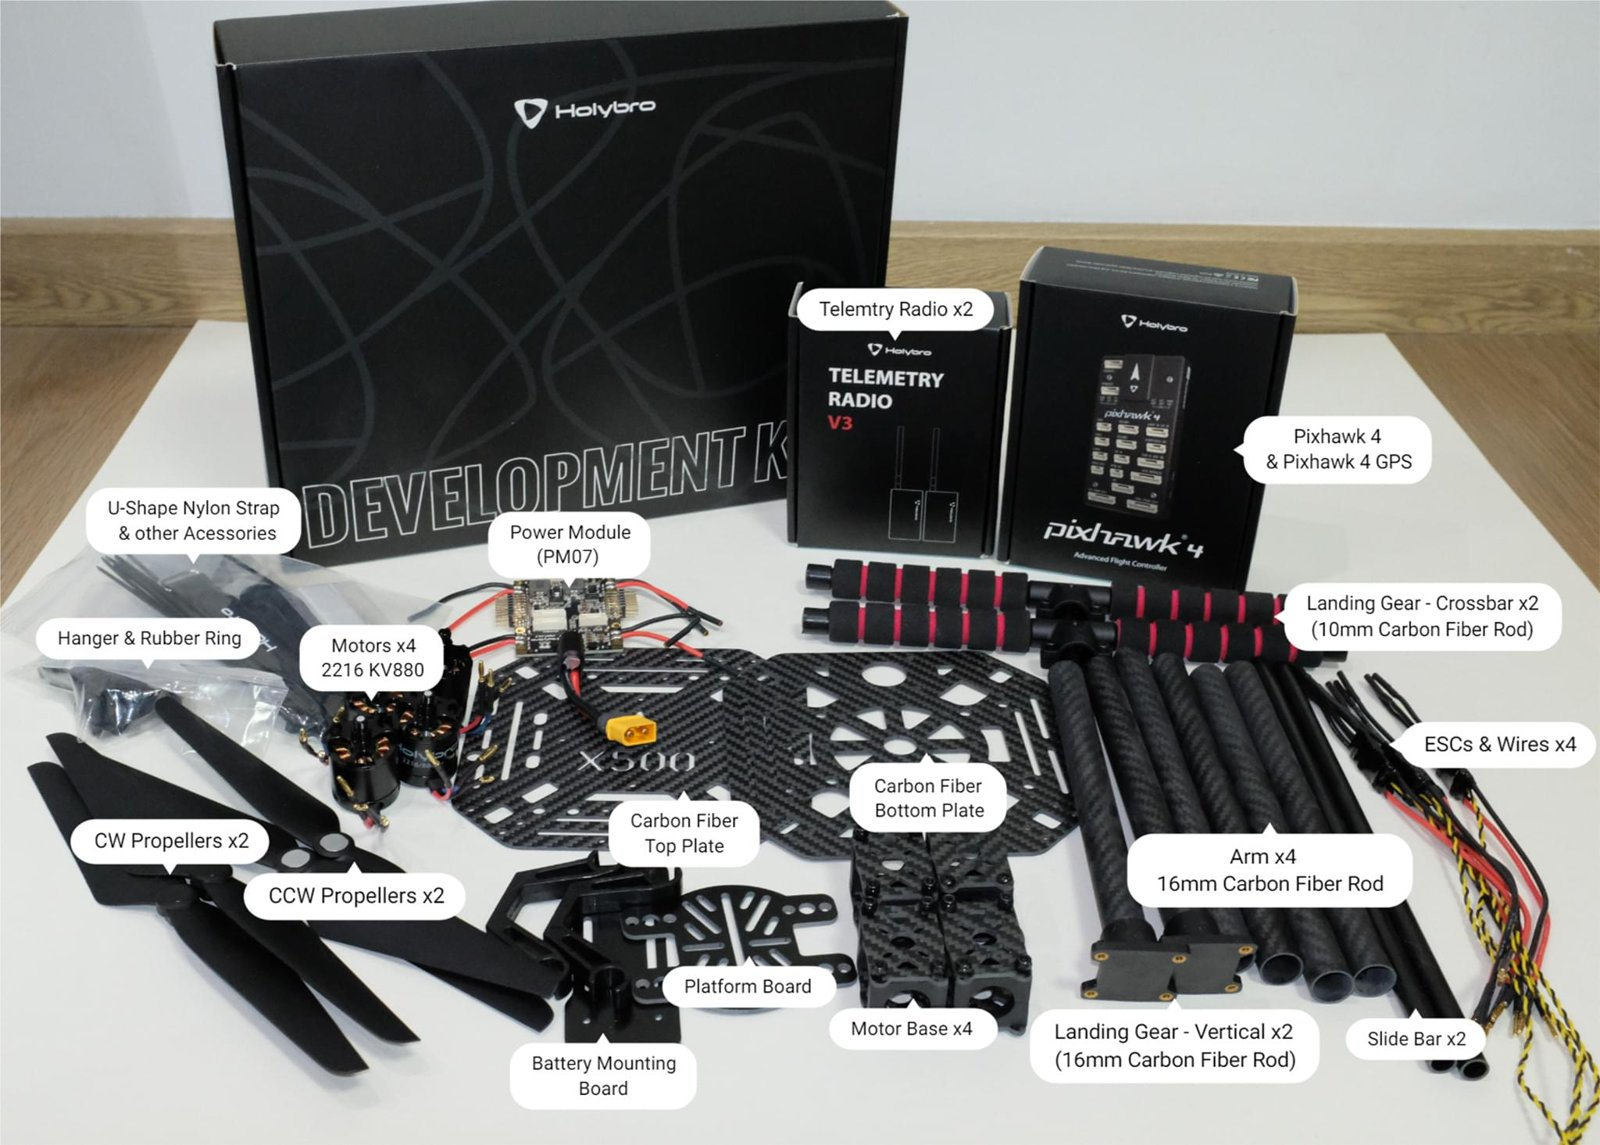
\includegraphics[height=0.78\textheight]{x500_kit_etiquetado}\\
  \credito{El kit del X500 desarmado, cada pieza con su nombre. Foto: documentación de PX4 (CC BY 4.0)}
\end{frame}

\begin{frame}{Las piezas, de un vistazo}
  \centering
  \begin{tikzpicture}[every node/.style={font=\scriptsize,align=center},
      pz/.style={draw=azul,fill=azulclaro,rounded corners,minimum width=2.7cm,minimum height=1.1cm}]
    \node[pz,fill=yellow!25] (fc) at (0,0) {\textbf{Pixhawk}\\el cerebro (PX4)};
    \node[pz] (gps) at (-4.2,1.6) {\textbf{GPS + brújula}\\dónde está};
    \node[pz] (esc) at (4.2,1.6) {\textbf{4 ESC + motores}\\los músculos};
    \node[pz] (bat) at (-4.2,-1.6) {\textbf{Batería}\\la energía};
    \node[pz] (rad) at (4.2,-1.6) {\textbf{Radio de telemetría}\\habla con QGC};
    \node[pz] (pc) at (0,2.4) {\textbf{Computadora a bordo}\\aquí corre ROS 2};
    \node[pz] (rc) at (0,-2.4) {\textbf{Receptor RC}\\el control del piloto};
    \foreach \n in {gps,esc,bat,rad,pc,rc} \draw[{Stealth}-{Stealth},thick,gris] (fc) -- (\n);
  \end{tikzpicture}
\end{frame}

\begin{frame}{El cerebro: la Pixhawk 6C}
  \begin{columns}[c]
    \column{0.4\textwidth}\centering
    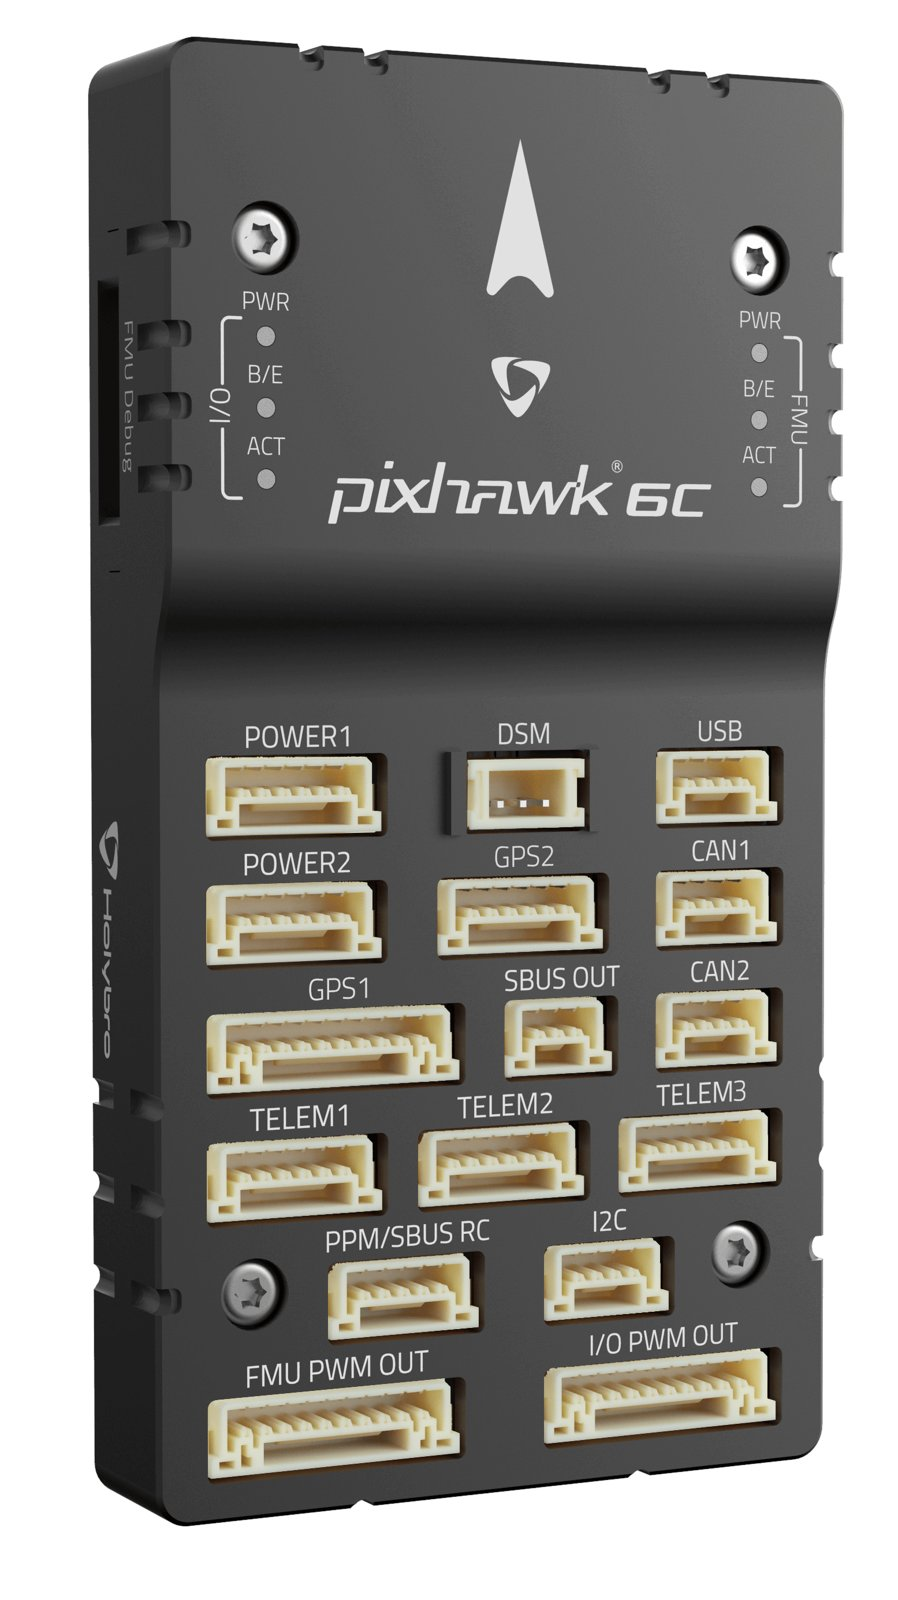
\includegraphics[height=0.62\textheight]{pixhawk6c}\\
    \credito{Foto: documentación de PX4 (CC BY 4.0)}
    \column{0.57\textwidth}\small
    \begin{itemize}
      \item Una computadora pequeña dedicada a \textbf{volar}. Ahí corre \textbf{PX4}.
      \item Trae adentro la \textbf{IMU} (giroscopio y acelerómetro) y el \textbf{barómetro}.
      \item Decide cuánto girar cada motor, \textbf{cientos de veces por segundo}.
      \item Nosotros no la programamos por dentro: le \textbf{pedimos} cosas desde ROS 2.
    \end{itemize}
    \begin{idea}
      \small En ROS 2 la IMU aparece como \cmd{/fmu/out/sensor\_combined} y lo que PX4 sabe del dron como
      \cmd{/fmu/out/vehicle\_status\_v1}.
    \end{idea}
  \end{columns}
\end{frame}

\begin{frame}{Tiene un frente}
  \begin{columns}[c]
    \column{0.4\textwidth}\centering
    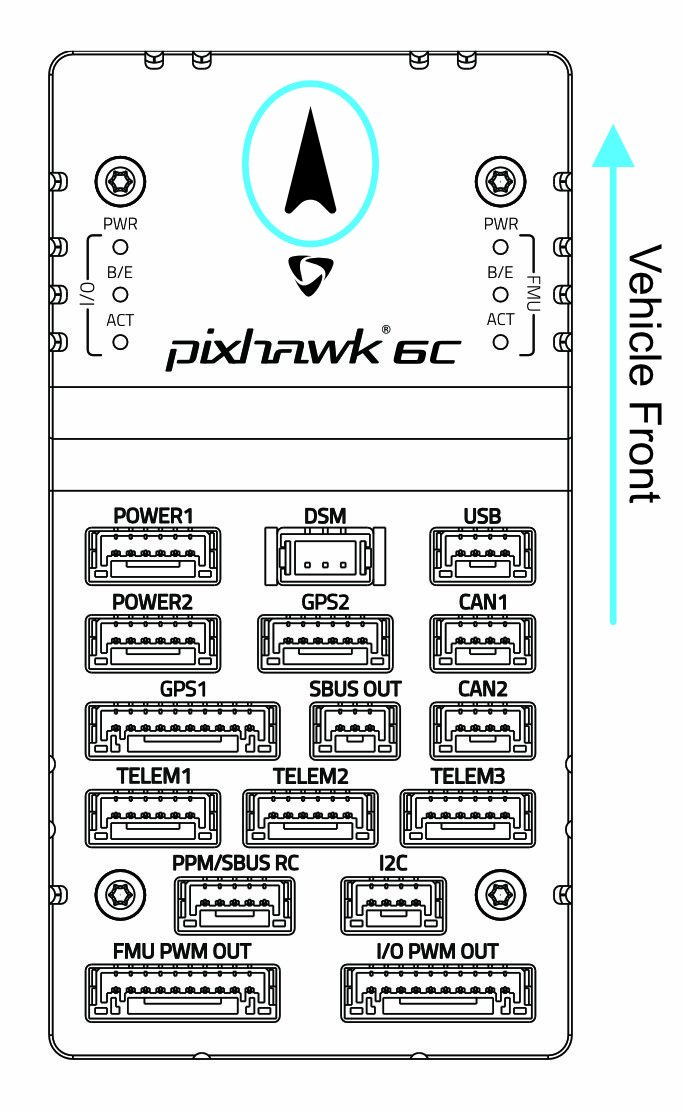
\includegraphics[height=0.62\textheight]{pixhawk6c_frente}\\
    \credito{Foto: documentación de PX4 (CC BY 4.0)}
    \column{0.57\textwidth}\small
    \begin{itemize}
      \item La flecha de la Pixhawk tiene que apuntar al \textbf{frente del dron}.
      \item PX4 mide todo respecto a ella: si la montas al revés, cree que avanza cuando retrocede.
      \item En PX4 ese marco se llama \textbf{FRD}: x al \textbf{F}rente, y a la de\textbf{R}echa,
        z hacia a\textbf{D}entro de la tierra (abajo).
    \end{itemize}
  \end{columns}
\end{frame}

\begin{frame}{Dónde está: GPS y brújula}
  \begin{columns}[c]
    \column{0.36\textwidth}\centering
    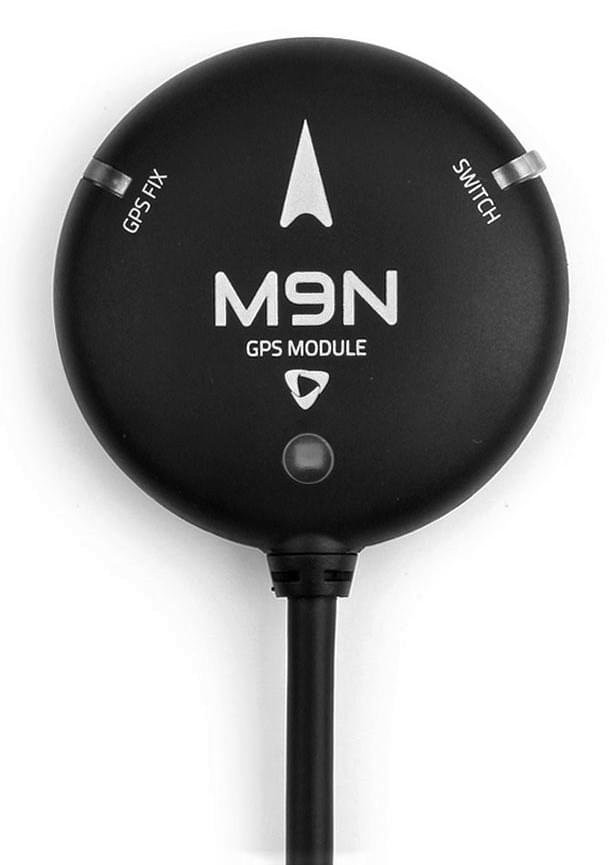
\includegraphics[height=0.6\textheight]{gps_m9n}\\
    \credito{Holybro M9N. Foto: documentación de PX4 (CC BY 4.0)}
    \column{0.6\textwidth}\small
    \begin{itemize}
      \item El \textbf{GPS} da latitud y longitud (unos 5--10 veces por segundo, con \textasciitilde1 m de error).
      \item Trae una \textbf{brújula} (magnetómetro): sabe hacia dónde está el norte.
      \item Va arriba, en un mástil, lejos de los cables (los motores hacen ``ruido'' magnético).
    \end{itemize}
    \begin{idea}
      \small En ROS 2: el GPS crudo en \cmd{/fmu/out/vehicle\_gps\_position}, y la posición que PX4 calcula
      combinando todo en \cmd{/fmu/out/vehicle\_global\_position}.
    \end{idea}
  \end{columns}
\end{frame}

\begin{frame}{Los músculos: motores, ESC y hélices}
  \begin{columns}[c]
    \column{0.45\textwidth}\centering
    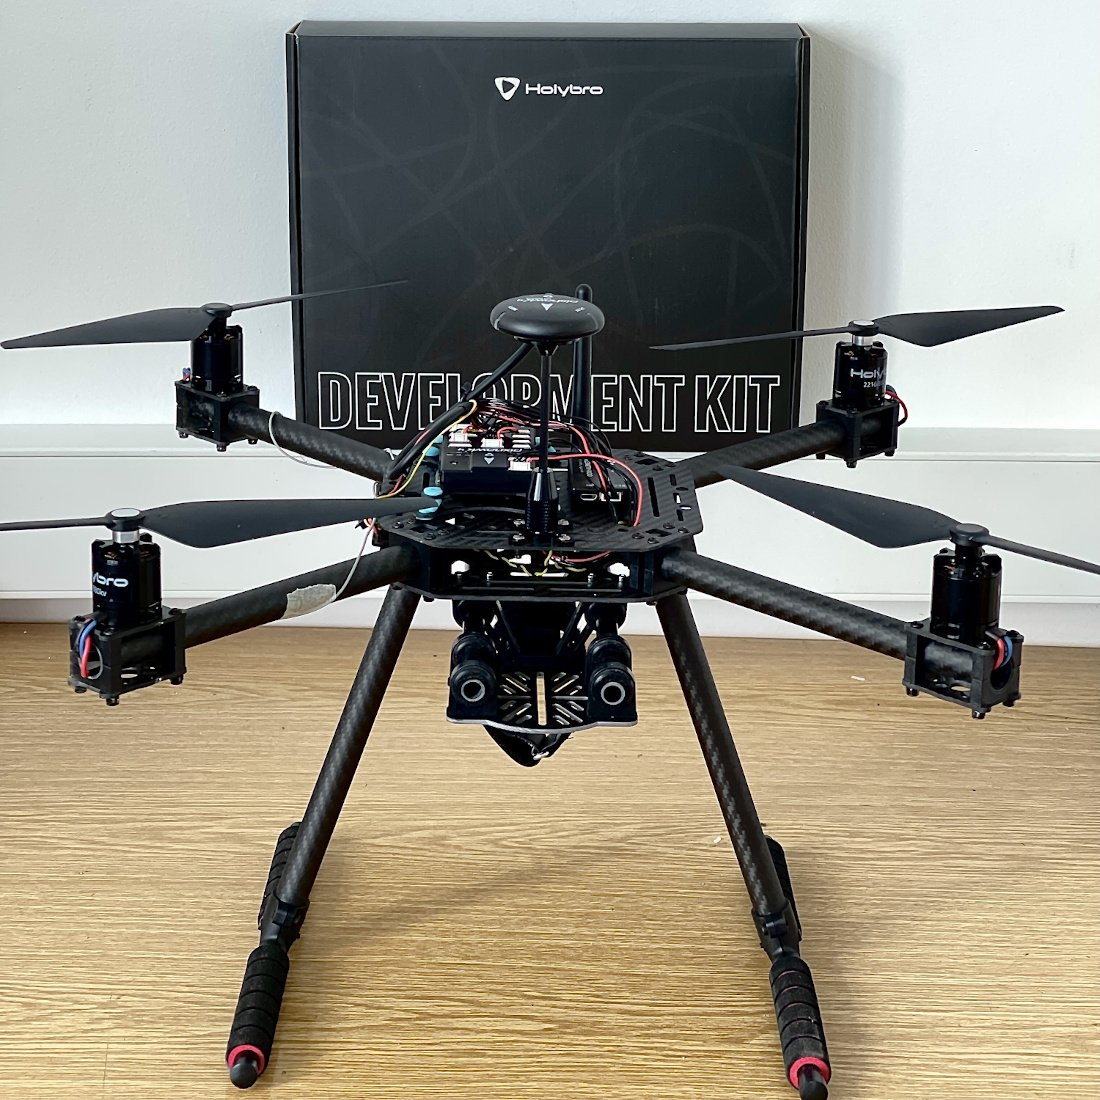
\includegraphics[width=\linewidth]{x500_armado}\\
    \credito{Foto: documentación de PX4 (CC BY 4.0)}
    \column{0.52\textwidth}\small
    \begin{itemize}
      \item Cada brazo lleva un \textbf{motor} sin escobillas con su \textbf{hélice}.
      \item Cada motor tiene un \textbf{ESC}: el ``traductor'' entre la orden de la Pixhawk (``75 \%'') y la
        corriente que mueve el motor.
      \item Dos giran a un lado y dos al otro (luego vemos por qué).
    \end{itemize}
    \begin{ojo}
      \small Las hélices cortan. Toda prueba de motores en el dron real va \textbf{sin hélices}.
    \end{ojo}
  \end{columns}
\end{frame}

\begin{frame}{Energía y comunicación}
  \begin{columns}[t]
    \column{0.48\textwidth}\small
    \textbf{Batería LiPo (4S)}
    \begin{itemize}
      \item 4 celdas de \textasciitilde4.2 V llenas: \textasciitilde16.8 V.
      \item Un vuelo dura minutos: hay que vigilarla.
      \item En ROS 2: \cmd{/fmu/out/battery\_status\_v1}.
    \end{itemize}
    \vspace{0.3em}
    \textbf{Control remoto (RC)}
    \begin{itemize}
      \item El piloto de seguridad: puede tomar el control en cualquier momento.
    \end{itemize}
    \column{0.48\textwidth}\centering
    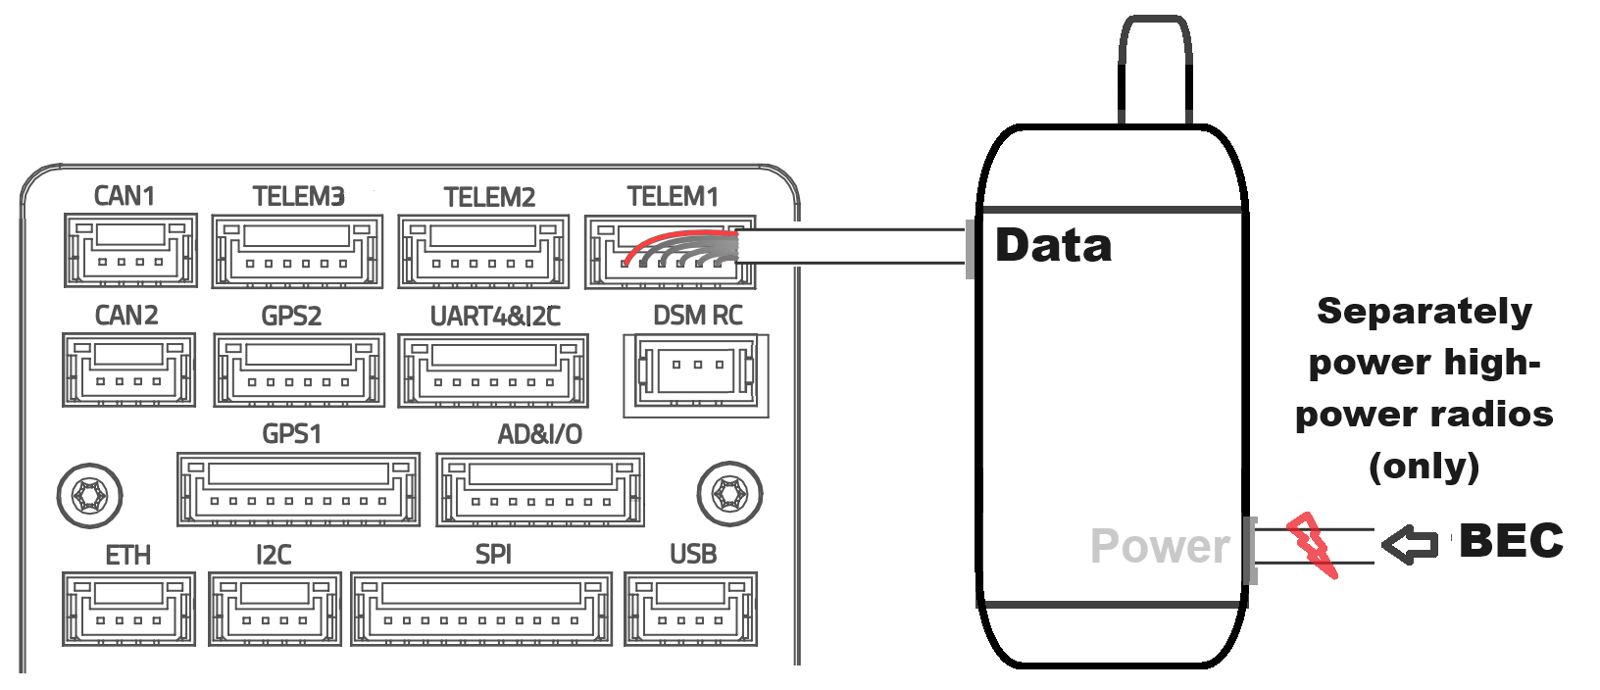
\includegraphics[width=\linewidth]{telemetria_conexion}\\
    \credito{Radio de telemetría conectada a la Pixhawk. Documentación de PX4 (CC BY 4.0)}\\[0.3em]
    \raggedright\small La \textbf{radio de telemetría} conecta el dron con \textbf{QGroundControl} en tu laptop.
  \end{columns}
\end{frame}

\begin{frame}{De la pieza al topic}
  \centering\small
  \begin{tabular}{lll}
    \toprule
    En el dron & Lo que mide o hace & En ROS 2 lo lees en \\
    \midrule
    IMU (en la Pixhawk) & giros y aceleraciones & \cmd{/fmu/out/sensor\_combined} \\
    GPS & latitud, longitud & \cmd{/fmu/out/vehicle\_gps\_position} \\
    PX4 combinando todo & dónde está, en metros & \cmd{/fmu/out/vehicle\_local\_position\_v1} \\
    PX4 combinando todo & hacia dónde apunta & \cmd{/fmu/out/vehicle\_attitude} \\
    Batería & voltaje, \% & \cmd{/fmu/out/battery\_status\_v1} \\
    PX4 (el piloto) & armado, modo de vuelo & \cmd{/fmu/out/vehicle\_status\_v1} \\
    \midrule
    Motores (vía PX4) & a dónde ir & \cmd{/fmu/in/trajectory\_setpoint} \\
    PX4 (el piloto) & órdenes: armar, aterrizar\ldots & \cmd{/fmu/in/vehicle\_command} \\
    \bottomrule
  \end{tabular}
  \vspace{0.4em}

  \raggedright\small \cmd{out} = PX4 nos cuenta. \cmd{in} = le pedimos algo.
\end{frame}

% =============================================================================
\section{Su gemelo en la simulación}
% =============================================================================

\begin{frame}{El mismo dron, en la computadora}
  \begin{columns}[c]
    \column{0.48\textwidth}\centering
    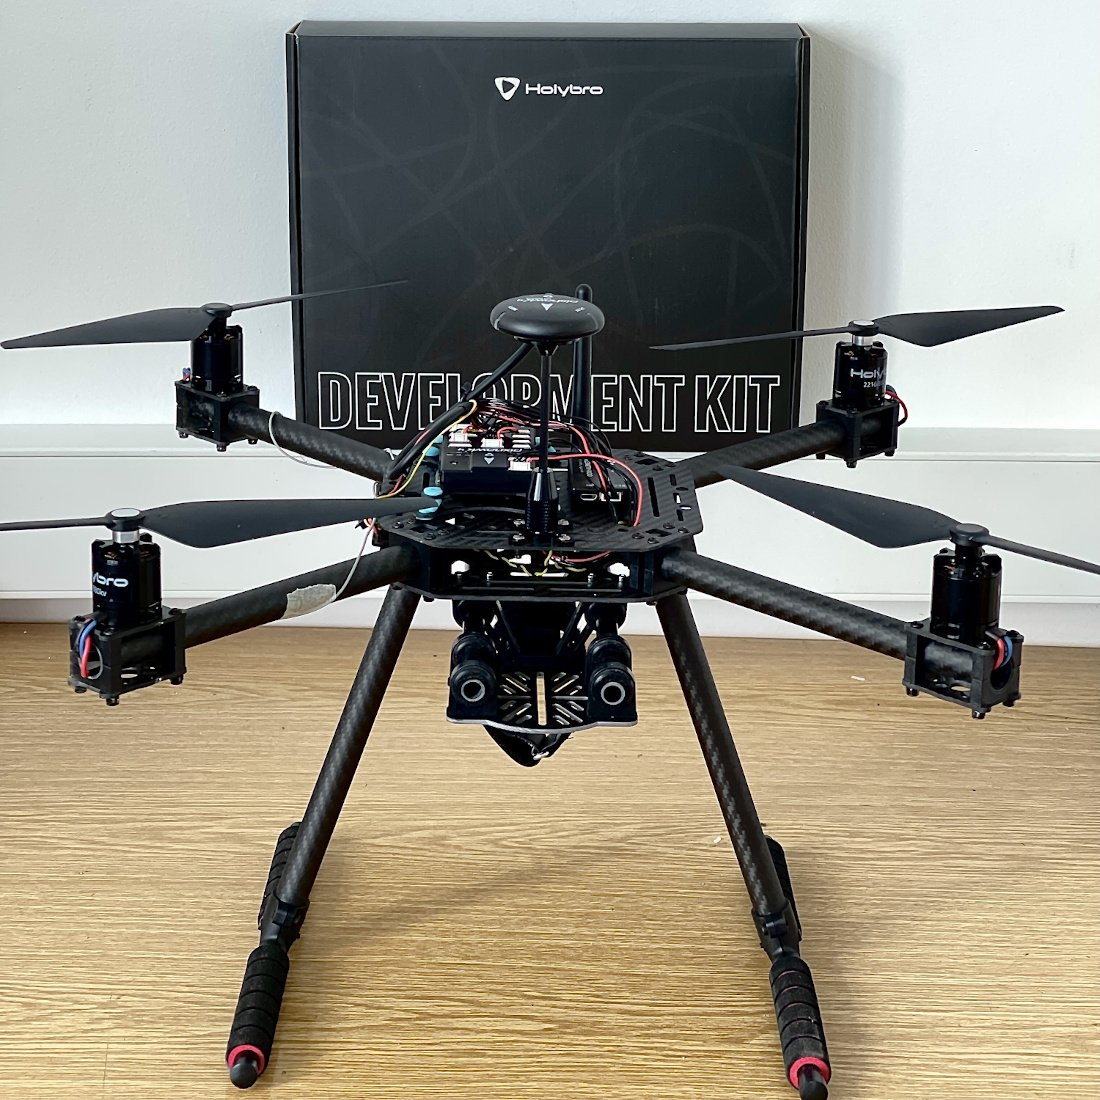
\includegraphics[width=\linewidth]{x500_armado}\\
    {\small\textbf{Real}}\\
    \credito{Foto: documentación de PX4 (CC BY 4.0)}
    \column{0.48\textwidth}\centering
    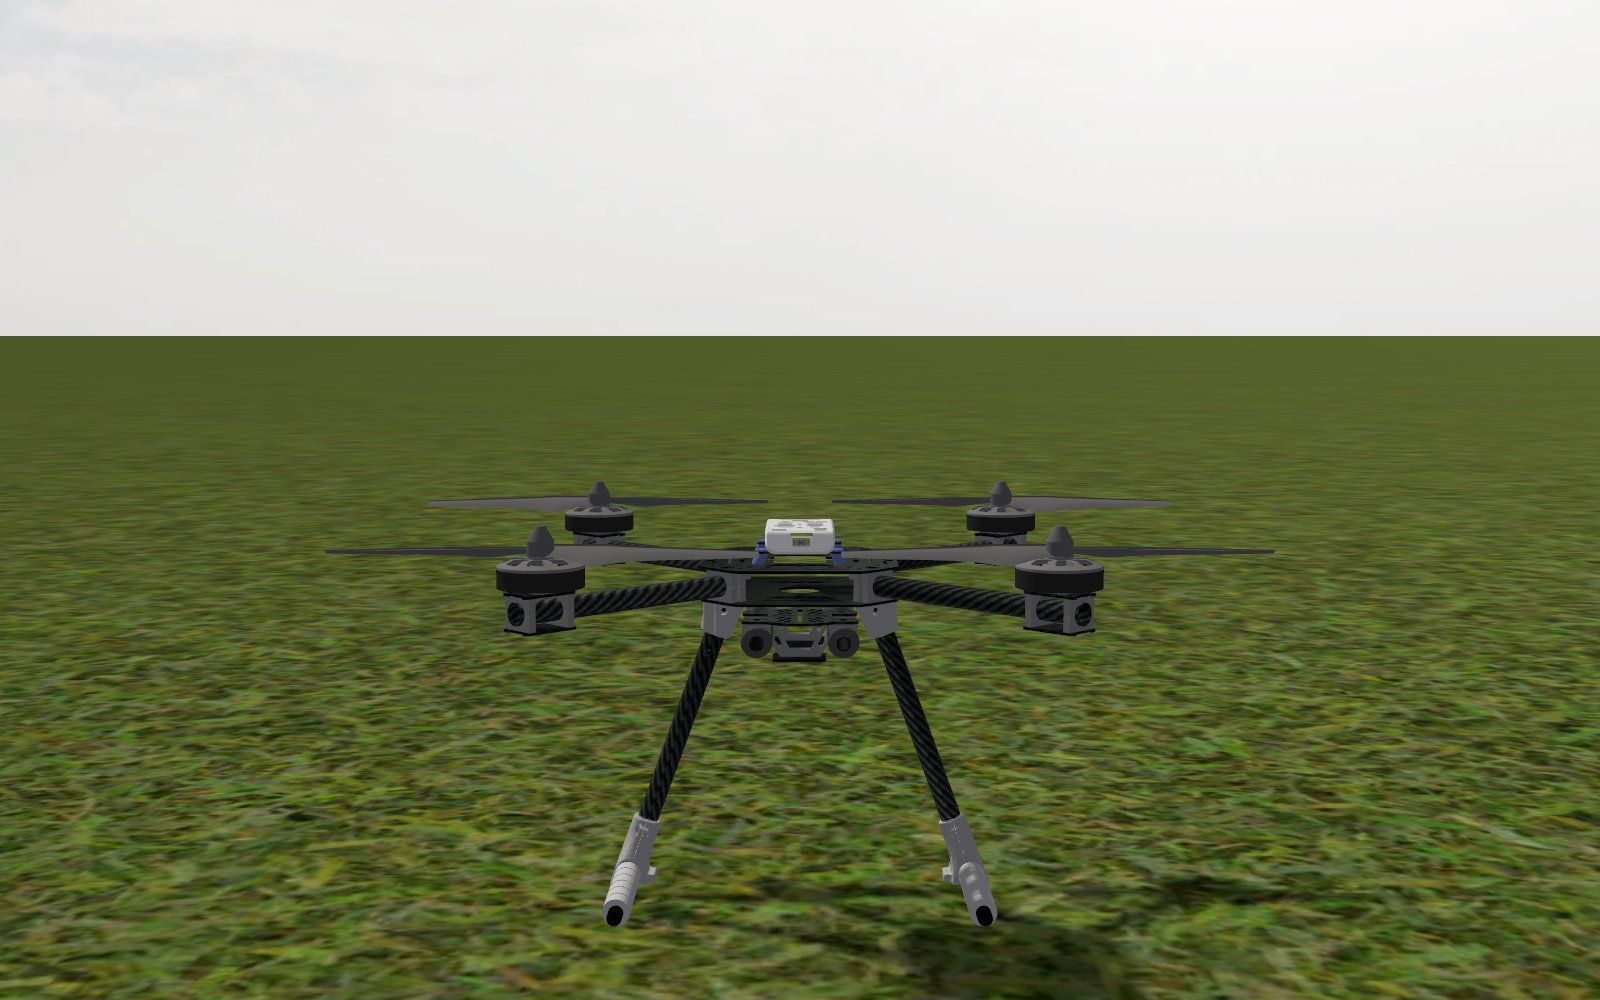
\includegraphics[width=\linewidth]{x500_frente}\\
    {\small\textbf{En Gazebo}}\\
    \credito{Render propio de Gazebo}
  \end{columns}
  \vspace{0.3em}
  \begin{idea}
    \small Gazebo simula la física (gravedad, empuje, viento) y los sensores. PX4 corre \textbf{el mismo
    programa} que en la Pixhawk. Tu nodo no sabe si habla con el real o con el simulado.
  \end{idea}
\end{frame}

\begin{frame}{Visto de cerca}
  \centering
  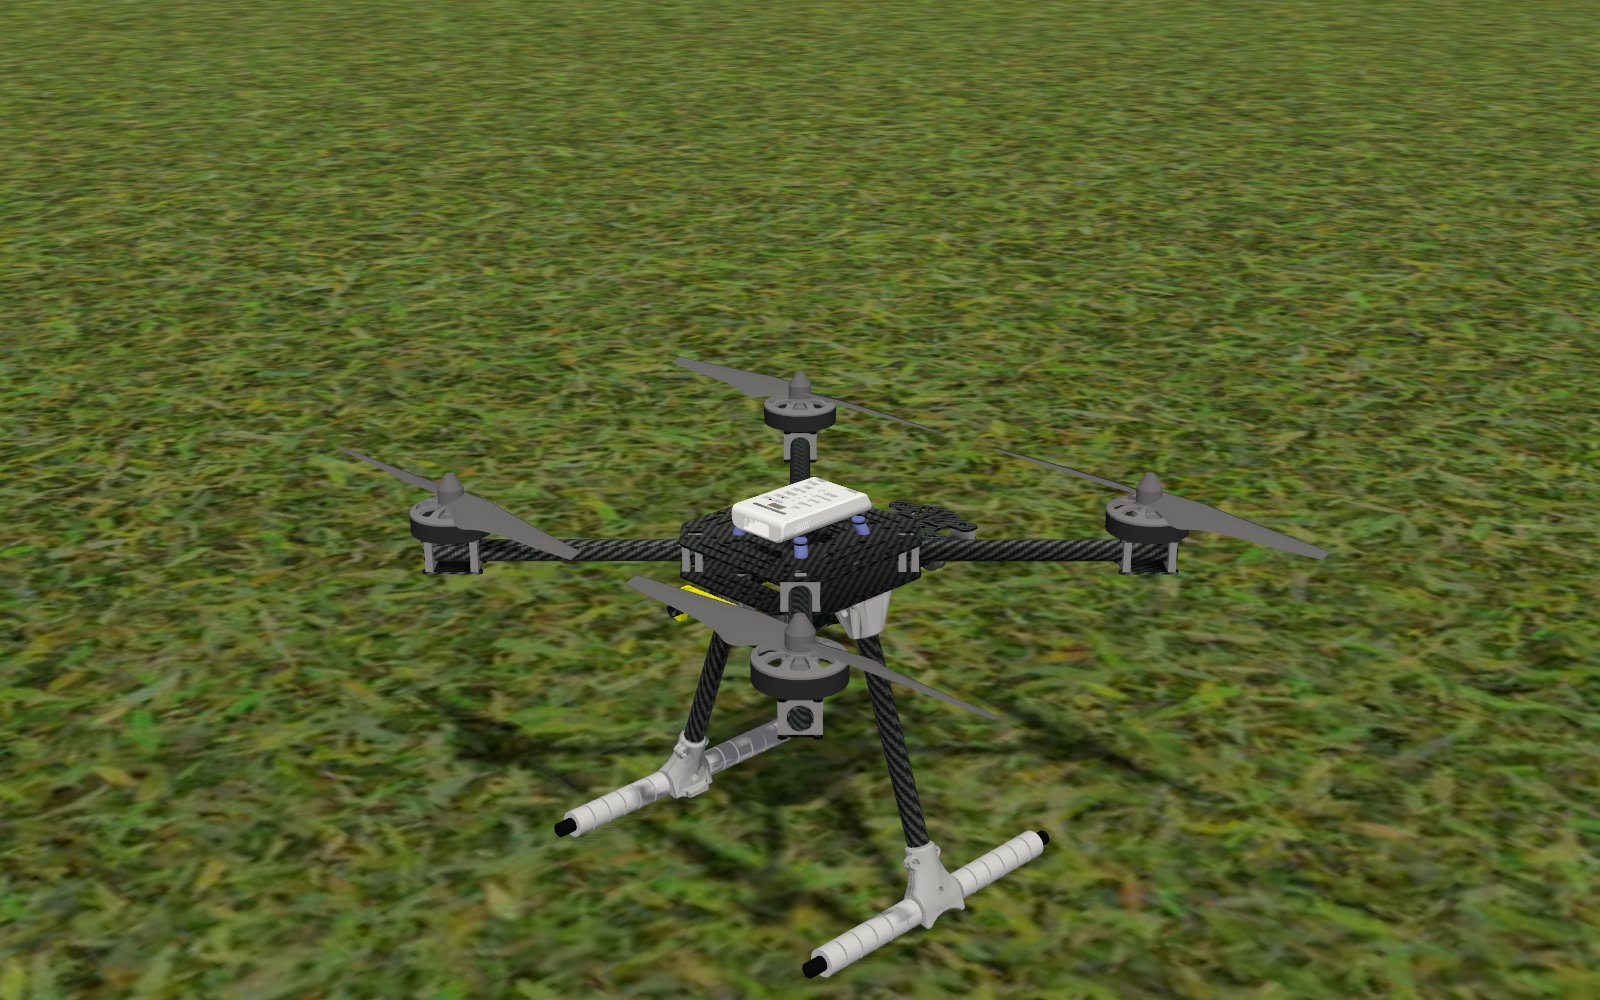
\includegraphics[height=0.8\textheight]{x500_tres_cuartos}\\
  \credito{El x500 de la simulación de PX4. Render propio de Gazebo}
\end{frame}

\begin{frame}{Los motores, desde arriba}
  \begin{columns}[c]
    \column{0.5\textwidth}\centering
    \begin{tikzpicture}
      \node[anchor=south west,inner sep=0] (img) at (0,0) {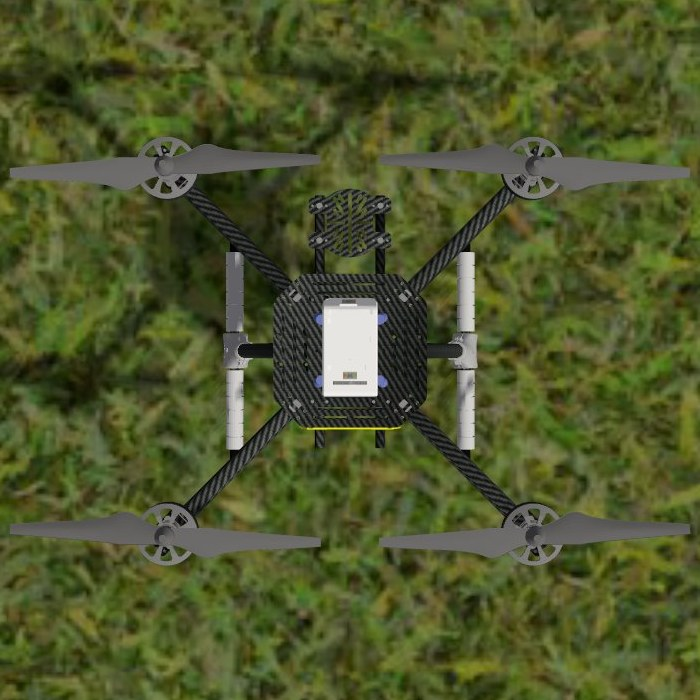
\includegraphics[height=0.75\textheight]{x500_arriba_recorte}};
      \begin{scope}[x={(img.south east)},y={(img.north west)}]
        % posición de cada motor en la foto (fracción de la imagen; el frente va arriba)
        \node[circle,fill=azul,text=white,font=\bfseries,inner sep=2.5pt] at (0.757,0.771) {1};
        \node[circle,fill=azul,text=white,font=\bfseries,inner sep=2.5pt] at (0.236,0.25) {2};
        \node[circle,fill=rojo,text=white,font=\bfseries,inner sep=2.5pt] at (0.236,0.771) {3};
        \node[circle,fill=rojo,text=white,font=\bfseries,inner sep=2.5pt] at (0.757,0.25) {4};
        \draw[-{Stealth},line width=2pt,verde] (0.5,0.62) -- (0.5,0.93);
        \node[font=\scriptsize\bfseries,verde,fill=white,inner sep=1pt] at (0.5,0.965) {FRENTE};
      \end{scope}
    \end{tikzpicture}
    \column{0.47\textwidth}\small
    \begin{itemize}
      \item {\color{azul}\textbf{1 y 2}} giran \textbf{antihorario}.
      \item {\color{rojo}\textbf{3 y 4}} giran \textbf{horario}.
      \item Los que giran igual van en diagonal: así sus ``torceduras'' se cancelan y el dron no da vueltas
        solo.
      \item Para \textbf{girar}, PX4 acelera un par y frena el otro.
    \end{itemize}
  \end{columns}
\end{frame}

\begin{frame}{Lo mismo en QGroundControl}
  \begin{columns}[c]
    \column{0.55\textwidth}\centering
    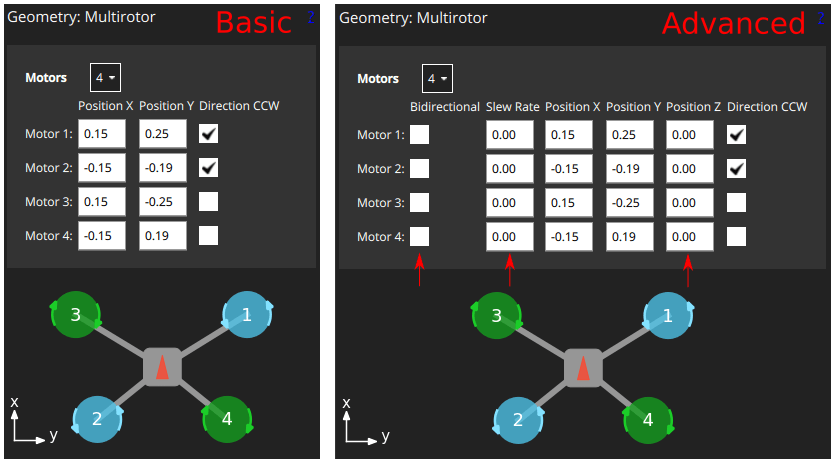
\includegraphics[width=\linewidth]{qgc_motores}\\
    \credito{Pantalla de motores de QGroundControl. Documentación de PX4 (CC BY 4.0)}
    \column{0.42\textwidth}\small
    \begin{itemize}
      \item QGC dibuja el mismo orden: el triángulo rojo es el frente.
      \item Ahí se prueba cada motor en el dron real (o con \cmd{motor\_test} desde ROS 2).
      \item Si dos motores están cruzados, \textbf{el dron se voltea al despegar}.
    \end{itemize}
  \end{columns}
\end{frame}

\begin{frame}{Con sensores extra}
  \begin{columns}[t]
    \column{0.48\textwidth}\centering
    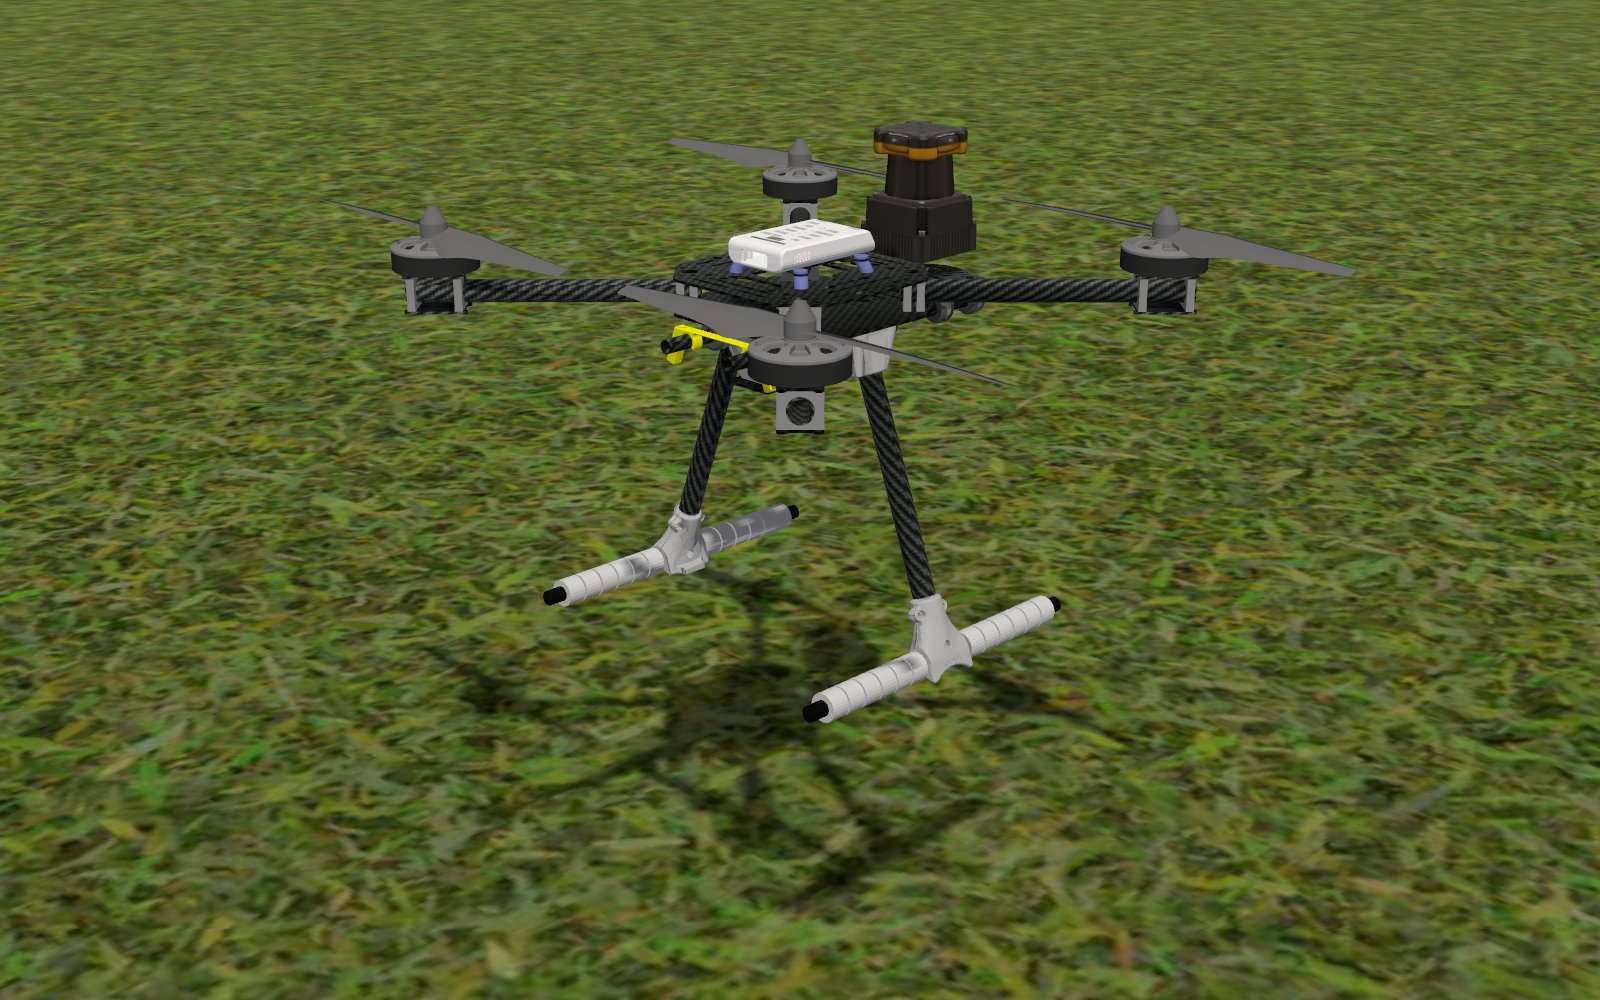
\includegraphics[width=\linewidth]{x500_lidar}\\
    {\small\textbf{x500\_lidar\_2d}}: un lidar arriba que mide distancias a 360$^\circ$ (como un radar de luz).
    \column{0.48\textwidth}\centering
    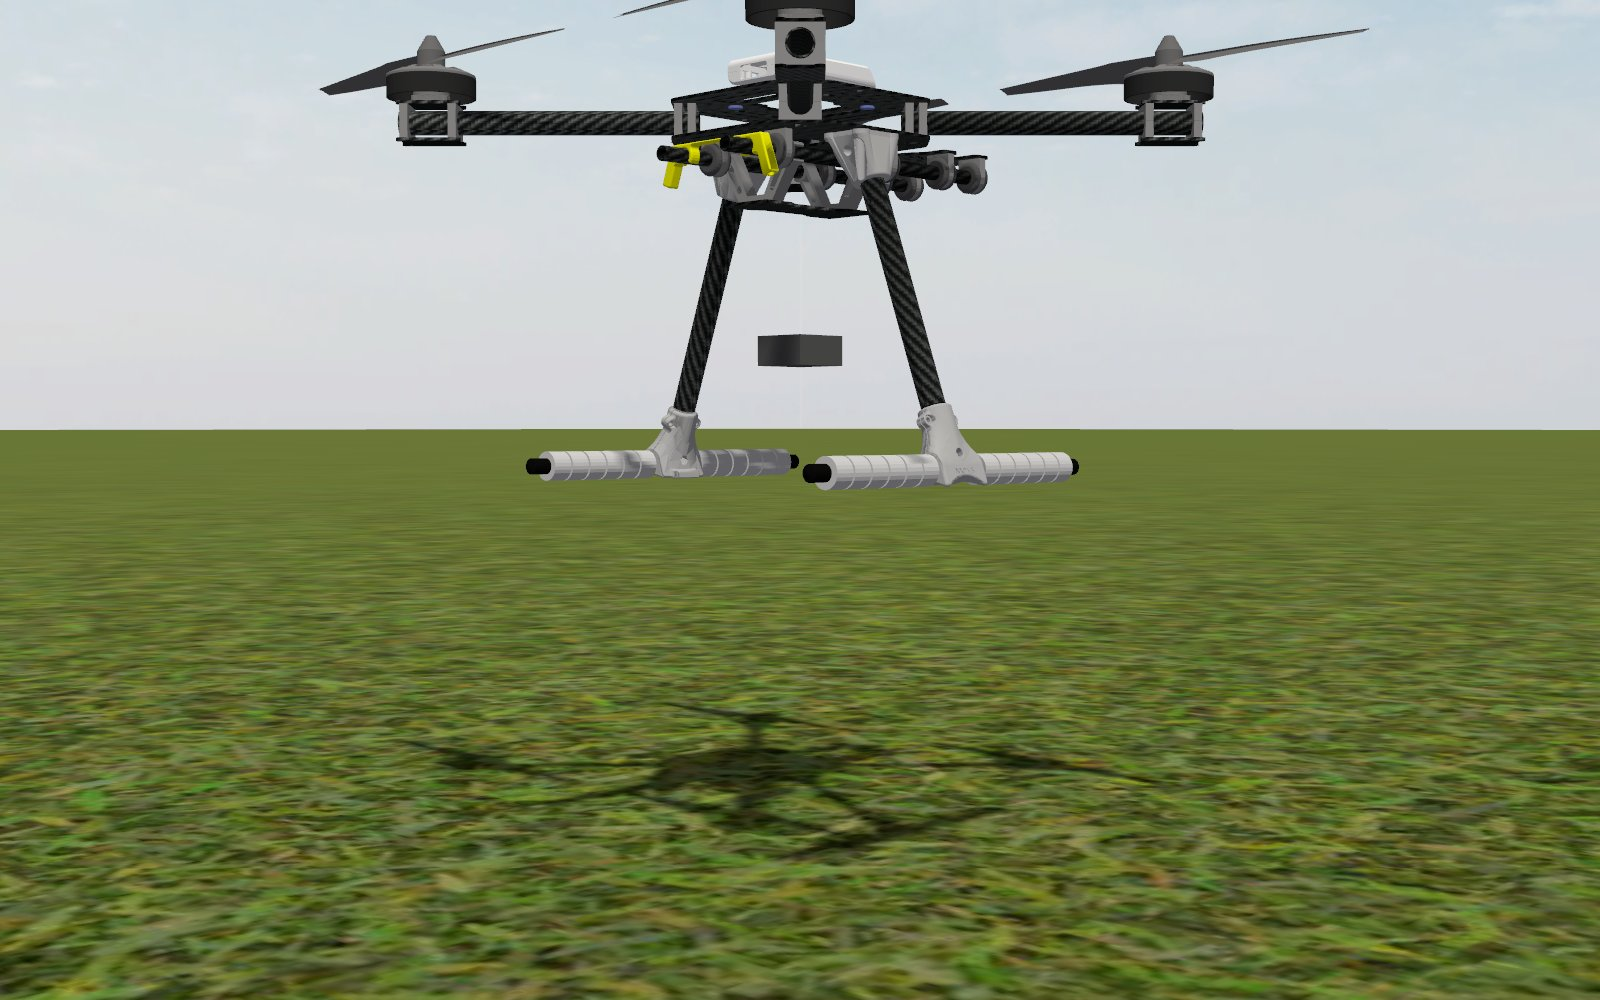
\includegraphics[width=\linewidth]{x500_cam_abajo}\\
    {\small\textbf{x500\_cam\_abajo}}: una cámara que mira hacia el suelo, para buscar marcadores.
  \end{columns}
  \vspace{0.2em}
  \centering\credito{Renders propios de Gazebo}
\end{frame}

% =============================================================================
\section{Quién hace qué}
% =============================================================================

\begin{frame}{Cuatro programas, cuatro papeles}
  \centering
  \begin{tikzpicture}[every node/.style={font=\scriptsize,align=center},
      ch/.style={draw=azul,fill=azulclaro,rounded corners,text width=3.1cm,minimum height=2.2cm}]
    \node[ch,fill=yellow!20] (n) at (0,0) {\textbf{Tu nodo de ROS 2}\\[0.2em]\emph{el copiloto}\\[0.2em]decide la misión:\\``sube a 5 m'', ``ve allá''};
    \node[ch] (p) at (4.3,0) {\textbf{PX4}\\[0.2em]\emph{el piloto}\\[0.2em]mantiene el dron en el aire\\y obedece al copiloto};
    \node[ch,fill=gray!10,draw=gray] (g) at (8.6,0) {\textbf{Gazebo}\\[0.2em]\emph{el mundo}\\[0.2em]gravedad, viento,\\sensores (en simulación)};
    \node[ch,fill=gray!10,draw=gray] (q) at (4.3,-2.9) {\textbf{QGroundControl}\\[0.2em]\emph{la torre de control}\\[0.2em]ve todo, puede tomar\\el control};
    \draw[-{Stealth},thick] (n) -- node[above]{pide} (p);
    \draw[{Stealth}-{Stealth},thick] (p) -- node[above]{motores / sensores} (g);
    \draw[{Stealth}-{Stealth},thick] (p) -- (q);
  \end{tikzpicture}
\end{frame}

\begin{frame}{El piloto y el copiloto}
  \begin{columns}[c]
    \column{0.55\textwidth}\small
    Piensen en un avión:
    \begin{itemize}
      \item El \textbf{piloto} (PX4) tiene las manos en los controles: mantiene el equilibrio, corrige el
        viento, nunca suelta.
      \item El \textbf{copiloto} (tu nodo) lleva el mapa y le dice a dónde ir: ``sube a 5 m'', ``ahora al
        norte''.
      \item Si el copiloto se desmaya (tu nodo se cae), el piloto \textbf{no se estrella}: hace lo seguro
        (quedarse quieto, regresar o aterrizar).
    \end{itemize}
    \column{0.42\textwidth}
    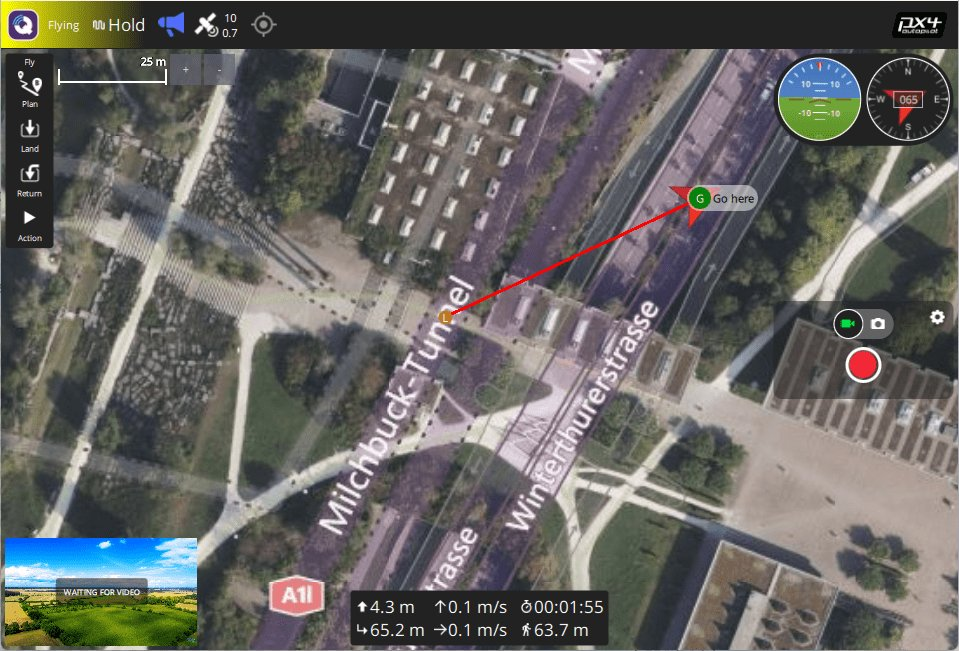
\includegraphics[width=\linewidth]{qgc_fly_view}\\
    \credito{QGroundControl, vista de vuelo. Documentación de PX4 (CC BY 4.0)}
  \end{columns}
\end{frame}

\begin{frame}{Dos formas de darle instrucciones al piloto}
  \begin{columns}[t]
    \column{0.48\textwidth}
    \begin{idea}[title={\small\bfseries ``Sigue mi mano'' (offboard)},coltitle=black,colbacktitle=azulclaro]
      \small El copiloto dice \textbf{a cada instante} dónde estar: 10--20 veces por segundo.
      \begin{itemize}
        \item Para trayectorias propias: un círculo, un 8, seguir algo.
        \item Si deja de hablar medio segundo, el piloto toma el control.
      \end{itemize}
    \end{idea}
    \column{0.48\textwidth}
    \begin{idea}[title={\small\bfseries ``Ve a tal lugar'' (comandos)},coltitle=black,colbacktitle=azulclaro]
      \small El copiloto da una \textbf{orden} y espera: ``despega'', ``ve a este punto GPS'', ``regresa''.
      \begin{itemize}
        \item El piloto vuela con sus propias maniobras.
        \item Si el copiloto se calla, el piloto se queda quieto.
      \end{itemize}
    \end{idea}
  \end{columns}
\end{frame}

% =============================================================================
\section{El viaje de un comando}
% =============================================================================

\begin{frame}{El viaje de un comando: ``sube a 5 metros''}
  \centering
  \begin{tikzpicture}[every node/.style={font=\scriptsize,align=center},
      st/.style={draw=azul,rounded corners,minimum width=2.1cm,minimum height=0.95cm}]
    \node[st,alt=<1>{fill=yellow!40}{fill=azulclaro}] (a) at (0,0) {\textbf{1} Tu nodo\\publica};
    \node[st,alt=<2>{fill=yellow!40}{fill=azulclaro}] (b) at (2.75,0) {\textbf{2} El agente\\traduce};
    \node[st,alt=<3>{fill=yellow!40}{fill=azulclaro}] (c) at (5.5,0) {\textbf{3} PX4\\recibe};
    \node[st,alt=<4>{fill=yellow!40}{fill=azulclaro}] (d) at (8.25,0) {\textbf{4} Los motores\\aceleran};
    \node[st,alt=<5>{fill=yellow!40}{fill=azulclaro}] (e) at (11,0) {\textbf{5} El dron\\sube};
    \node[st,alt=<6>{fill=yellow!40}{fill=azulclaro}] (f) at (8.25,-1.6) {\textbf{6} Los sensores\\lo notan};
    \node[st,alt=<7>{fill=yellow!40}{fill=azulclaro}] (g) at (2.75,-1.6) {\textbf{7} Tu nodo lee\\la altura};
    \foreach \x/\y in {a/b,b/c,c/d,d/e} \draw[-{Stealth},thick] (\x) -- (\y);
    \draw[-{Stealth},thick] (e) |- (f); \draw[-{Stealth},thick] (f) -- (g); \draw[-{Stealth},thick] (g) -| (a);
  \end{tikzpicture}
  \vspace{0.3em}

  \begin{columns}[c]
    \column{0.42\textwidth}\centering
    \only<1>{\begin{terminal}{ros2 run px4\_examples takeoff\_mission}
Comandos OFFBOARD + ARM enviados\\
alt=0.04 m
    \end{terminal}}%
    \only<2>{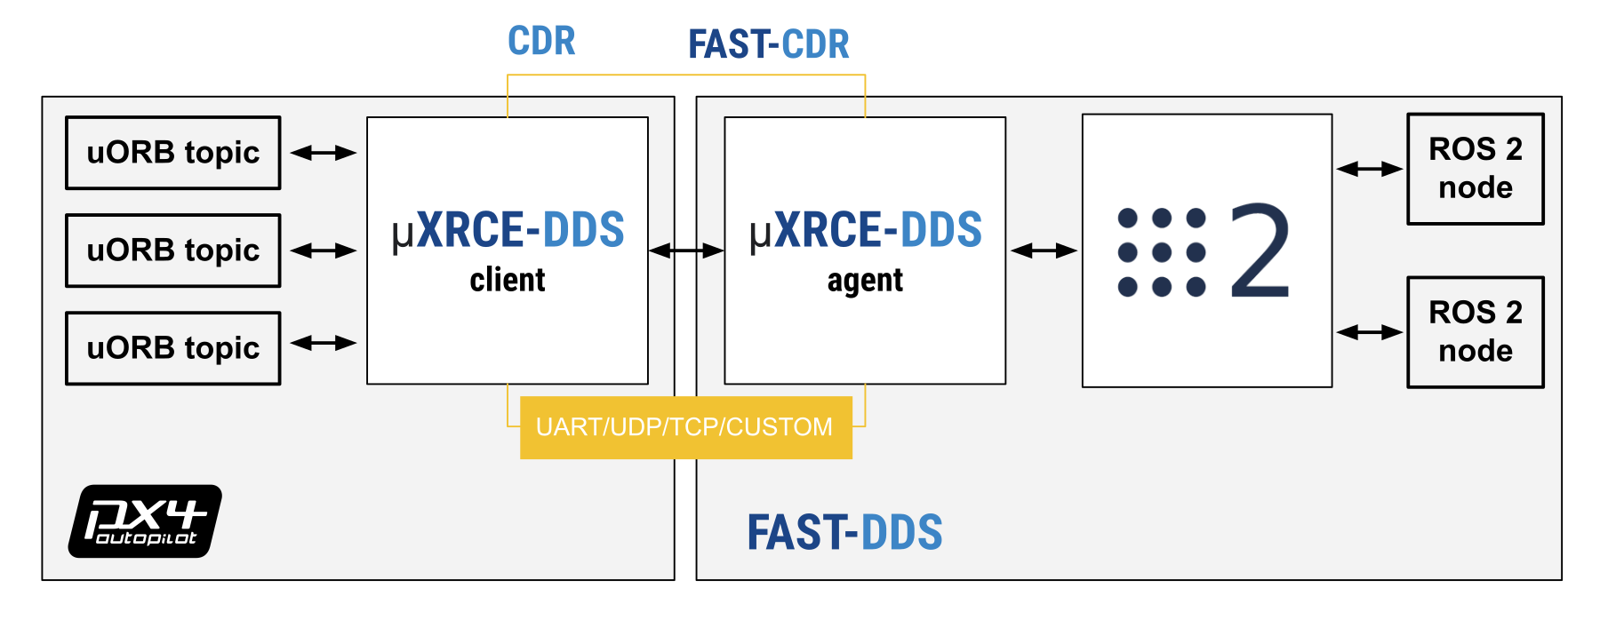
\includegraphics[width=\linewidth]{xrce_dds}\\\credito{Documentación de PX4 (CC BY 4.0)}}%
    \only<3>{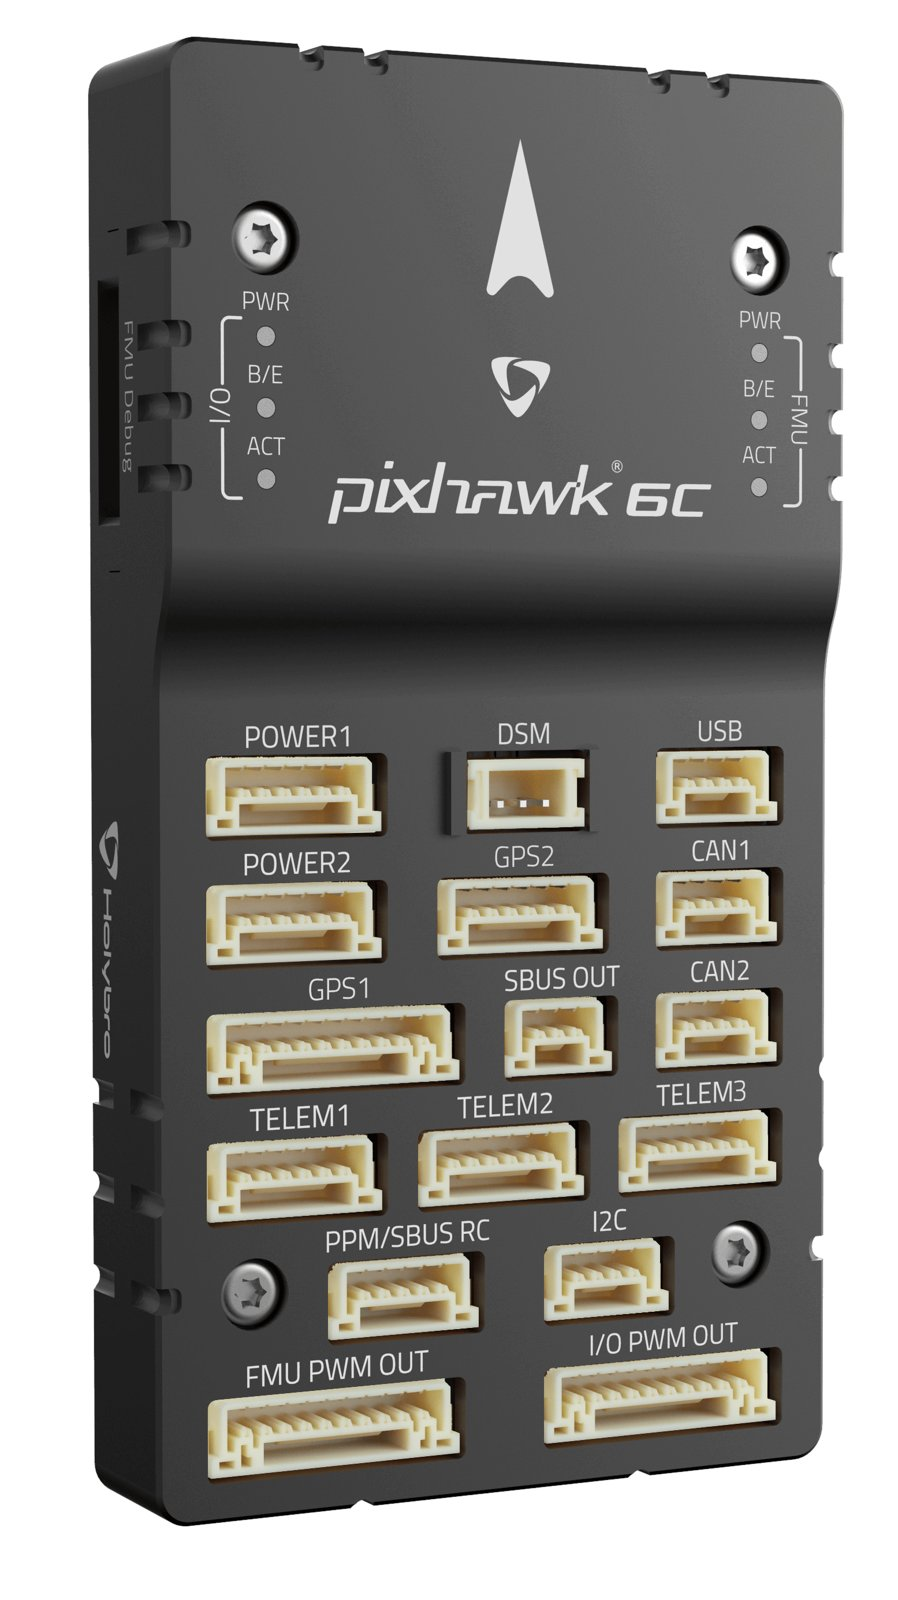
\includegraphics[height=3.2cm]{pixhawk6c}}%
    \only<4>{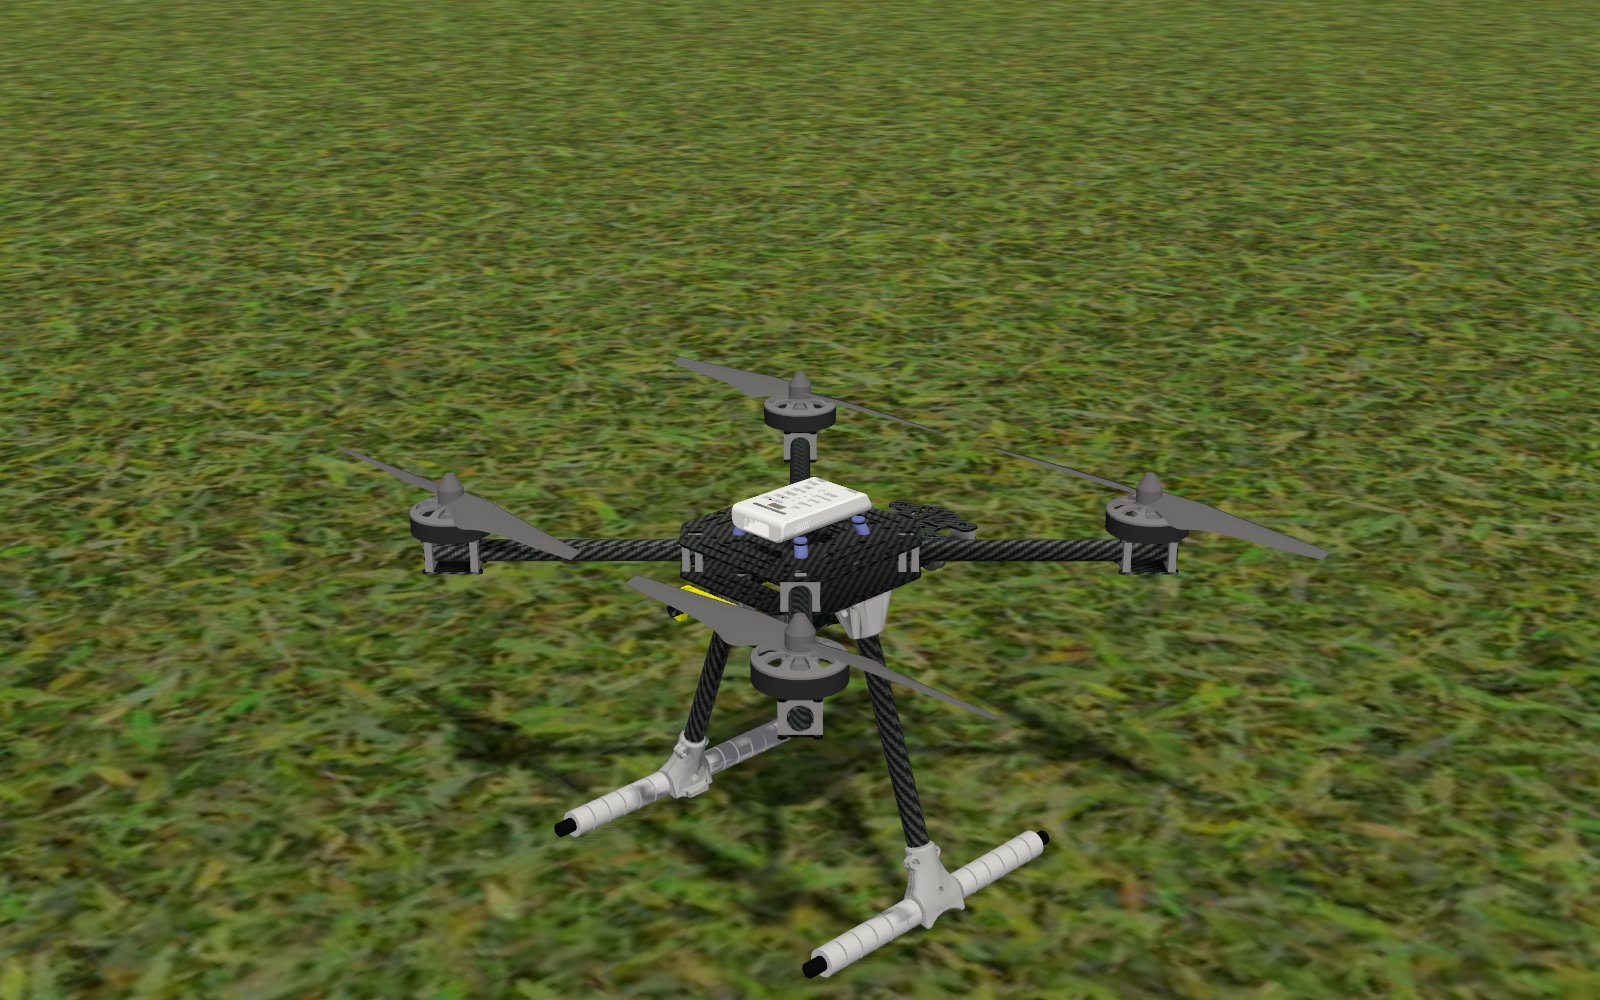
\includegraphics[width=\linewidth]{x500_tres_cuartos}}%
    \only<5>{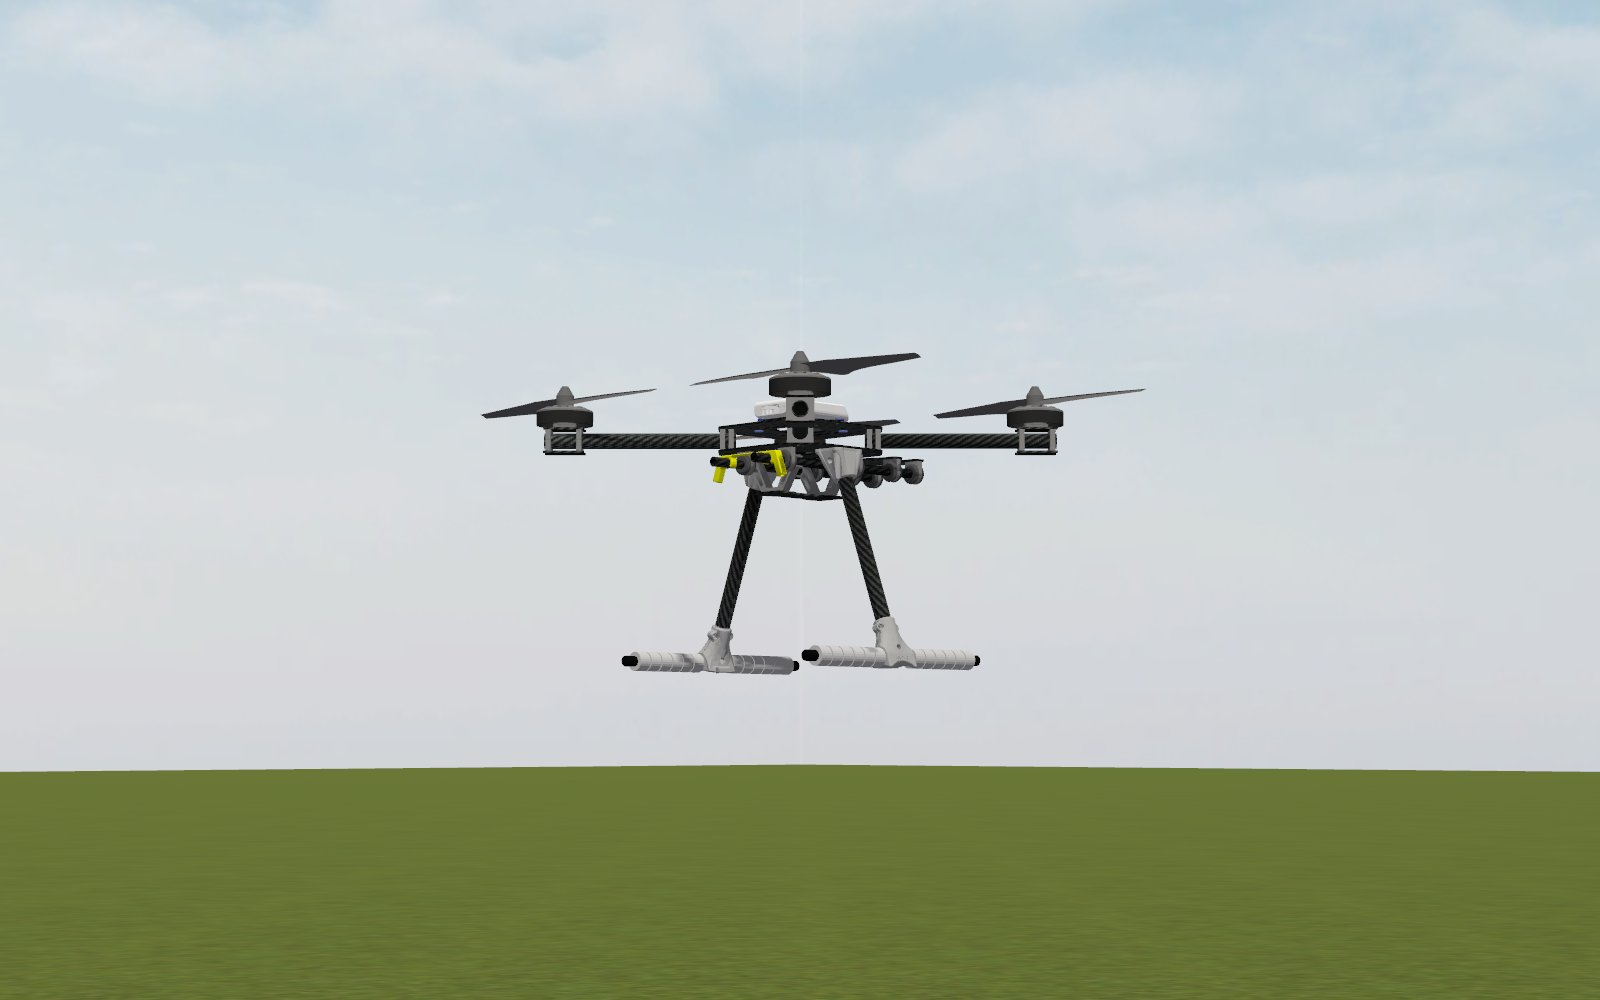
\includegraphics[width=\linewidth]{x500_volando}}%
    \only<6>{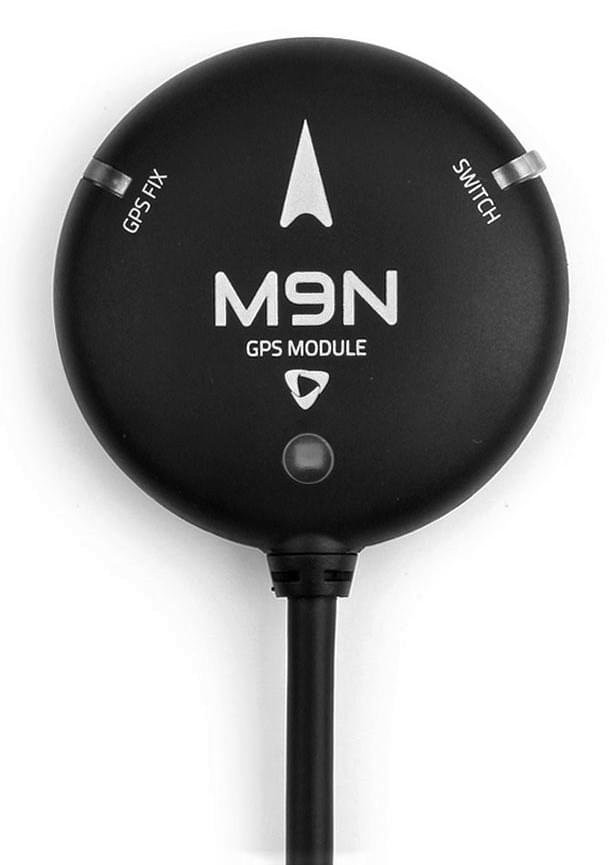
\includegraphics[height=3.2cm]{gps_m9n}}%
    \only<7>{\begin{terminal}{takeoff\_mission}
alt=4.98 m\\
Arriba: mantengo 5 m
    \end{terminal}}%
    \column{0.55\textwidth}\small
    \only<1>{Corres el programa. 10 veces por segundo publica un \textbf{setpoint}: ``quiero estar en
      $(0, 0, -5)$''. Al segundo pide \textbf{modo offboard} y \textbf{armar}.}%
    \only<2>{El \textbf{agente} (MicroXRCEAgent) toma los mensajes de ROS 2 y se los pasa a PX4 por UDP (en
      el dron real, por un cable serial).}%
    \only<3>{\textbf{PX4} revisa que todo esté bien (sensores, GPS, batería), \textbf{arma} y entra a
      \textbf{offboard}: desde ahora obedece tus setpoints.}%
    \only<4>{Los controladores de PX4 calculan cuánto empuje necesita cada motor para subir sin inclinarse,
      \textbf{cientos de veces por segundo}.}%
    \only<5>{En la simulación, \textbf{Gazebo} aplica ese empuje, la gravedad y el viento: el dron sube. En
      el real, lo hace la física.}%
    \only<6>{La IMU, el barómetro y el GPS miden el movimiento. El \textbf{EKF2} de PX4 los combina y
      calcula ``estoy a 4.98 m''.}%
    \only<7>{PX4 publica esa estimación en \cmd{vehicle\_local\_position\_v1}; tu nodo la lee y decide qué
      sigue. \textbf{Y el ciclo empieza otra vez.}}%
  \end{columns}
\end{frame}

\begin{frame}{Todo eso pasa 10 veces por segundo}
  \begin{columns}[c]
    \column{0.5\textwidth}\centering
    \begin{tikzpicture}[scale=1]
      \draw[azul!40,line width=8pt] (0,0) circle (1.6);
      \foreach \a/\t in {90/tu nodo,30/agente,-30/PX4,-90/motores,-150/sensores,150/EKF2} {
        \fill[white] (\a:1.6) circle (0.55); \draw[azul,thick] (\a:1.6) circle (0.55);
        \node[font=\tiny,align=center] at (\a:1.6) {\t};}
      \node[font=\scriptsize\bfseries] at (0,0) {100 ms};
    \end{tikzpicture}
    \column{0.47\textwidth}\small
    \begin{itemize}
      \item Tu nodo da una vuelta cada \textbf{100 ms} (un \emph{timer}).
      \item Por dentro, PX4 da \textbf{muchas más} vueltas: sus motores se ajustan cientos de veces entre
        uno de tus setpoints y el siguiente.
      \item Por eso tú solo dices \textbf{a dónde}, no cómo mover cada motor.
    \end{itemize}
  \end{columns}
\end{frame}

\begin{frame}{¿Y si tu nodo se cae?}
  \begin{columns}[c]
    \column{0.5\textwidth}\small
    En offboard, PX4 espera tus setpoints \textbf{todo el tiempo}. Es como el \textbf{pedal del hombre muerto} de
    los trenes: si el maquinista lo suelta, el tren frena solo.
    \begin{itemize}
      \item Si dejan de llegar setpoints (\textasciitilde0.5 s), PX4 entra en \textbf{failsafe}: se queda
        quieto, regresa o aterriza.
      \item Por eso el nodo publica aunque ``no cambie nada''.
    \end{itemize}
    \column{0.47\textwidth}
    \begin{terminal}{flight\_mode\_monitor (al dar Ctrl+C)}
Modo: Offboard -> Hold\\
FAILSAFE ACTIVO (modo Hold)\\
Banderas de failsafe:\\
\ \ señal offboard perdida
    \end{terminal}
  \end{columns}
\end{frame}

% =============================================================================
\section{Lo que vas a ver}
% =============================================================================

\begin{frame}[fragile]{Un comando levanta todo}
  \begin{lstlisting}[style=bash]
vespo up --sim
  \end{lstlisting}
  \centering
  \begin{tikzpicture}[every node/.style={font=\scriptsize,align=center},
      w/.style={draw=gray,fill=gray!8,rounded corners,minimum width=3.3cm,minimum height=1.6cm}]
    \node[w] (t1) at (0,0) {\textbf{Terminal: agente}\\MicroXRCEAgent\\(el traductor)};
    \node[w] (t2) at (4,0) {\textbf{Terminal: PX4}\\la consola \cmd{pxh>}\\(mensajes de PX4)};
    \node[w,fill=azulclaro,draw=azul] (gz) at (8,0) {\textbf{Ventana: Gazebo}\\el mundo y el dron};
    \node[w,fill=azulclaro,draw=azul] (qg) at (12,0) {\textbf{Ventana: QGC}\\mapa, modo, altura};
  \end{tikzpicture}
  \vspace{0.4em}
  \begin{columns}[c]
    \column{0.48\textwidth}\centering
    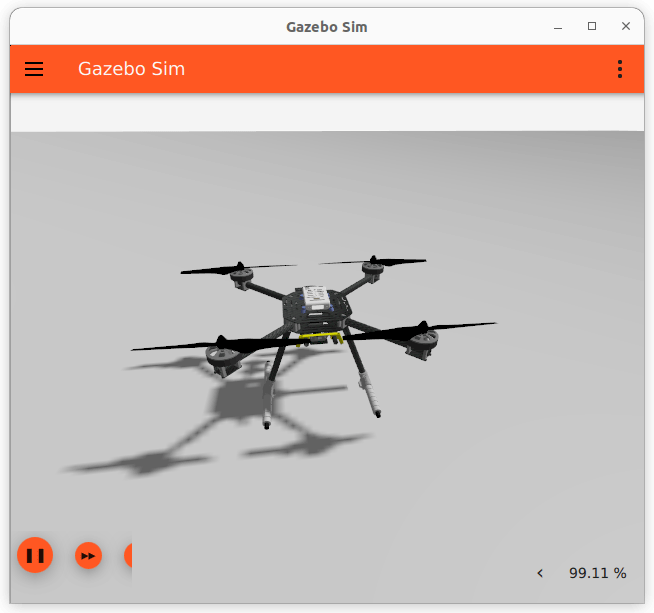
\includegraphics[height=3.3cm]{gazebo_x500}\\\credito{Gazebo. Documentación de PX4 (CC BY 4.0)}
    \column{0.48\textwidth}\centering
    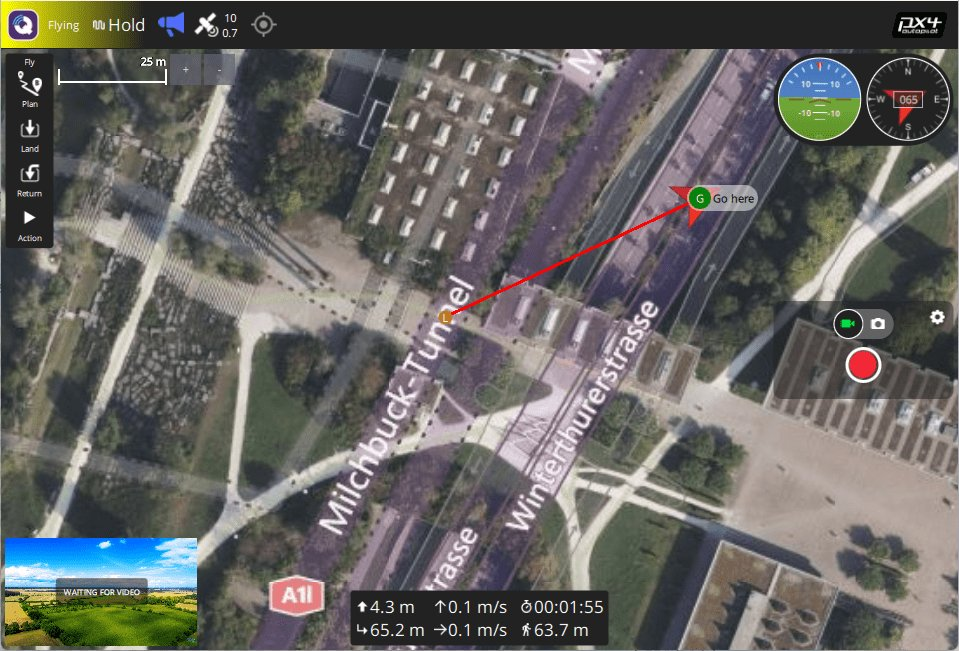
\includegraphics[height=3.3cm]{qgc_fly_view}\\\credito{QGroundControl. Documentación de PX4 (CC BY 4.0)}
  \end{columns}
\end{frame}

\begin{frame}{En QGroundControl, mira estas tres cosas}
  \begin{columns}[c]
    \column{0.58\textwidth}
    \begin{tikzpicture}
      \node[anchor=south west,inner sep=0] (img) at (0,0) {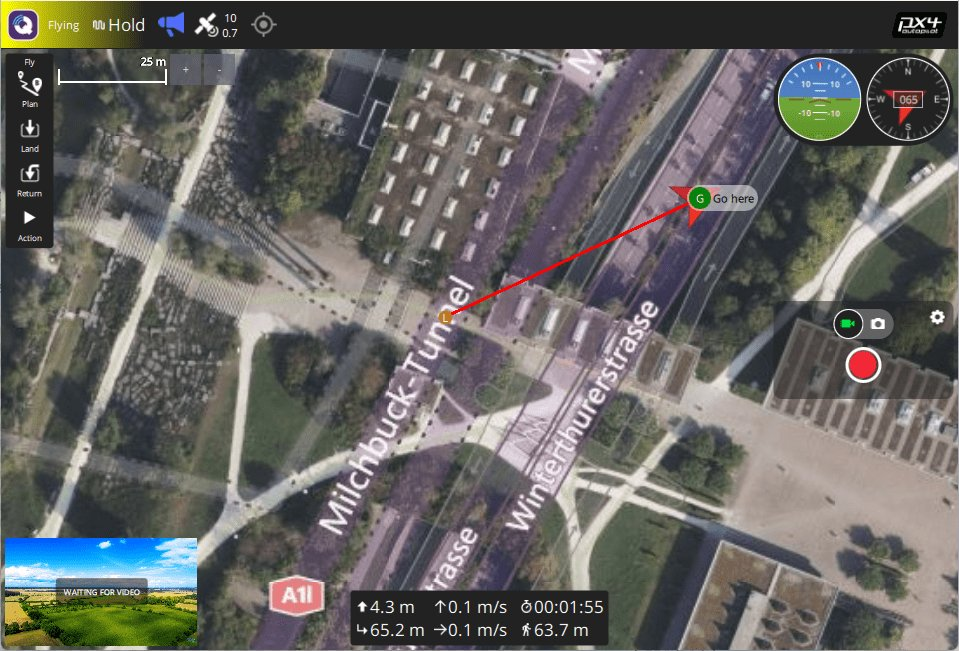
\includegraphics[width=\linewidth]{qgc_fly_view}};
      \begin{scope}[x={(img.south east)},y={(img.north west)}]
        \draw[rojo,line width=1.5pt,rounded corners] (0.0,0.93) rectangle (0.21,1.0);
        \node[circle,fill=rojo,text=white,font=\bfseries\scriptsize,inner sep=1.5pt] at (0.24,0.965) {1};
        \draw[rojo,line width=1.5pt,rounded corners] (0.37,0.02) rectangle (0.67,0.13);
        \node[circle,fill=rojo,text=white,font=\bfseries\scriptsize,inner sep=1.5pt] at (0.34,0.075) {2};
        \draw[rojo,line width=1.5pt,rounded corners] (0.0,0.6) rectangle (0.06,0.88);
        \node[circle,fill=rojo,text=white,font=\bfseries\scriptsize,inner sep=1.5pt] at (0.09,0.74) {3};
      \end{scope}
    \end{tikzpicture}\\
    \credito{Documentación de PX4 (CC BY 4.0)}
    \column{0.4\textwidth}\small
    \begin{enumerate}
      \item \textbf{Estado y modo}: ``Flying'', ``Hold'', ``Offboard''\ldots{} Lo primero que hay que ver
        cuando algo no jala.
      \item \textbf{Altura y velocidad}: la telemetría en vivo.
      \item \textbf{Botones de seguridad}: Land, Return\ldots{} el piloto siempre puede tomar el control.
    \end{enumerate}
  \end{columns}
\end{frame}

\begin{frame}{En la terminal}
  \begin{columns}[t]
    \column{0.48\textwidth}
    \begin{terminal}{ros2 run px4\_examples telemetry\_listener}
Estado: desarmado | modo: HOLD (4)\\
Local: x=0.01 y=-0.02 alt=0.03 m\\
GPS: lat=47.3979711 lon=8.5461637\\
Actitud: roll=0.1° pitch=-0.2° yaw=90.0°\\
Batería: 16.20 V | 100 \%
    \end{terminal}
    \small Si sale \textbf{``Sin datos de vehicle\_status todavía''}: el agente o PX4 no están corriendo.
    \column{0.48\textwidth}
    \begin{terminal}{ros2 topic list | grep fmu}
/fmu/in/offboard\_control\_mode\\
/fmu/in/trajectory\_setpoint\\
/fmu/in/vehicle\_command\\
/fmu/out/battery\_status\_v1\\
/fmu/out/vehicle\_local\_position\_v1\\
/fmu/out/vehicle\_status\_v1\\
\ldots
    \end{terminal}
  \end{columns}
\end{frame}

% =============================================================================
\section{Ideas para el código}
% =============================================================================

\begin{frame}{Un topic es una estación de radio}
  \begin{columns}[c]
    \column{0.5\textwidth}\centering
    \begin{tikzpicture}[every node/.style={font=\scriptsize,align=center}]
      \node[draw=azul,fill=azulclaro,rounded corners] (tx) at (0,0) {PX4\\(transmite)};
      \foreach \r in {0.5,0.8,1.1} \draw[naranja,thick] (0.9,0) ++(-40:\r) arc (-40:40:\r);
      \node[draw=gray,fill=gray!10,rounded corners] (r1) at (3.4,1.0) {telemetry\_listener};
      \node[draw=gray,fill=gray!10,rounded corners] (r2) at (3.4,0) {tu misión};
      \node[draw=gray,fill=gray!10,rounded corners] (r3) at (3.4,-1.0) {battery\_monitor};
      \node[font=\tiny,naranja] at (1.5,-1.2) {/fmu/out/vehicle\_status\_v1};
    \end{tikzpicture}
    \column{0.47\textwidth}\small
    \begin{itemize}
      \item El \textbf{publisher} transmite en una frecuencia con nombre (\cmd{/fmu/out/vehicle\_status\_v1}).
      \item Cualquier \textbf{subscriber} que sintonice ese nombre escucha. Pueden ser muchos.
      \item El que transmite no sabe quién escucha, ni le importa.
    \end{itemize}
  \end{columns}
\end{frame}

\begin{frame}{Radio en vivo o carta certificada (QoS)}
  \begin{columns}[t]
    \column{0.48\textwidth}
    \begin{idea}[title={\small\bfseries best\_effort: radio en vivo},coltitle=black,colbacktitle=azulclaro]
      \small Si te perdiste un mensaje, ya pasó; el siguiente llega en milisegundos. Así publica PX4: a 50 Hz
      no vale la pena repetir datos viejos.
    \end{idea}
    \column{0.48\textwidth}
    \begin{idea}[title={\small\bfseries reliable: carta certificada},coltitle=black,colbacktitle=azulclaro]
      \small Se reenvía hasta confirmar que llegó. Lo usamos entre nodos nuestros (\cmd{/vespo/...}).
    \end{idea}
  \end{columns}
  \vspace{0.5em}
  \begin{ojo}
    \small Si pides carta certificada a una estación de radio, \textbf{no te llega nada}. Por eso los ejemplos
    se suscriben a PX4 con \cmd{best\_effort}.
  \end{ojo}
\end{frame}

\begin{frame}{Un mensaje es un formulario}
  \begin{columns}[c]
    \column{0.45\textwidth}\centering
    \begin{tikzpicture}[every node/.style={font=\scriptsize,anchor=west}]
      \draw[fill=yellow!8,rounded corners] (0,0) rectangle (4.2,3.4);
      \node[font=\small\bfseries] at (0.2,3.05) {VehicleLocalPosition};
      \foreach \y/\c/\v in {2.45/x/1.20 m,1.95/y/0.80 m,1.45/z/$-$5.00 m,0.95/heading/0.00 rad,0.45/xy\_valid/true} {
        \node at (0.2,\y) {\c}; \draw (1.7,\y-0.18) rectangle (3.9,\y+0.18); \node at (1.75,\y) {\v};}
    \end{tikzpicture}
    \column{0.52\textwidth}\small
    \begin{itemize}
      \item Cada tipo de mensaje tiene sus \textbf{casillas} (campos) con nombre y tipo.
      \item PX4 llena el formulario y lo publica; tu nodo lo lee: \cmd{position\_.z}.
      \item Para ver las casillas de un tipo:\\ \cmd{ros2 interface show px4\_msgs/msg/VehicleLocalPosition}
    \end{itemize}
  \end{columns}
\end{frame}

\begin{frame}{NED: como un submarino}
  \begin{columns}[c]
    \column{0.45\textwidth}\centering
    \begin{tikzpicture}[scale=1.1]
      \draw[-{Stealth},thick,verde] (0,0) -- (0,1.7) node[above,font=\scriptsize] {Norte (x)};
      \draw[-{Stealth},thick,rojo] (0,0) -- (1.7,0) node[right,font=\scriptsize] {Este (y)};
      \draw[-{Stealth},thick,azul] (0,0) -- (0.9,-0.8) node[below right,font=\scriptsize] {Abajo (z)};
      \fill[naranja] (0,0) circle (2pt);
      \node[font=\tiny,below left] at (0,0) {despegue};
    \end{tikzpicture}
    \column{0.52\textwidth}\small
    PX4 mide como un submarino: ``cuántos metros al norte, al este y \textbf{de profundidad}''.
    \begin{itemize}
      \item $z = 0$: en el suelo donde arrancó.
      \item $z = -5$: \textbf{5 m arriba} (profundidad negativa).
      \item Por eso en los ejemplos la altura se calcula como \cmd{-z}.
    \end{itemize}
  \end{columns}
\end{frame}

\begin{frame}{Callbacks y timers: el timbre y la alarma}
  \begin{columns}[t]
    \column{0.48\textwidth}
    \begin{idea}[title={\small\bfseries Callback = el timbre},coltitle=black,colbacktitle=azulclaro]
      \small No te quedas en la puerta esperando el paquete: cuando llega, \textbf{suena el timbre} y ROS
      llama a tu función. En los ejemplos solo guarda el mensaje: \cmd{status\_ = *msg}.
    \end{idea}
    \column{0.48\textwidth}
    \begin{idea}[title={\small\bfseries Timer = la alarma},coltitle=black,colbacktitle=azulclaro]
      \small Suena cada 100 ms y llama a \cmd{loop()}: ahí se decide qué hacer con lo último que llegó y se
      publica el setpoint.
    \end{idea}
  \end{columns}
  \vspace{0.5em}
  \small Ninguno de los dos debe tardar: mientras uno corre, los demás esperan (un \cmd{sleep} adentro congela
  todo el nodo).
\end{frame}

\begin{frame}{SharedPtr: un documento compartido}
  \begin{columns}[c]
    \column{0.5\textwidth}\centering
    \begin{tikzpicture}[every node/.style={font=\scriptsize,align=center}]
      \draw[fill=yellow!15,rounded corners] (2.2,0.2) rectangle (4.6,1.6);
      \node at (3.4,1.1) {\textbf{el mensaje}};
      \node at (3.4,0.55) {abierto por: 3};
      \foreach \y/\n/\k in {1.9/callback A/a,0.9/callback B/b,-0.1/tu variable/c} {
        \node[draw=azul,fill=azulclaro,rounded corners] (p\k) at (0,\y) {\n};
        \draw[-{Stealth},thick] (p\k.east) -- (2.2,0.9);}
    \end{tikzpicture}
    \column{0.47\textwidth}\small
    \begin{itemize}
      \item Como un documento en la nube que varios tienen abierto: no se copia, todos ven el mismo.
      \item Lleva la cuenta de cuántos lo tienen abierto.
      \item Cuando el último lo cierra, \textbf{se borra solo}.
      \item Por eso en ROS 2 todo es \cmd{SharedPtr}: nadie tiene que acordarse de borrar nada.
    \end{itemize}
  \end{columns}
\end{frame}

% =============================================================================
\section{Tu primer vuelo}
% =============================================================================

\begin{frame}[fragile]{Paso 1: compilar y levantar}
  \begin{lstlisting}[style=bash]
cd /data/vespo_ws
vespo build                  # compila todo (la primera vez tarda)
vespo up --sim               # agente + PX4 + Gazebo + QGroundControl
  \end{lstlisting}
  \begin{columns}[c]
    \column{0.55\textwidth}\small
    Espera a que:
    \begin{itemize}
      \item Gazebo muestre el dron en el suelo,
      \item QGC diga \textbf{``Ready To Fly''} (puede tardar \textasciitilde30 s mientras el GPS simulado y el
        EKF2 se acomodan).
    \end{itemize}
    \column{0.42\textwidth}\centering
    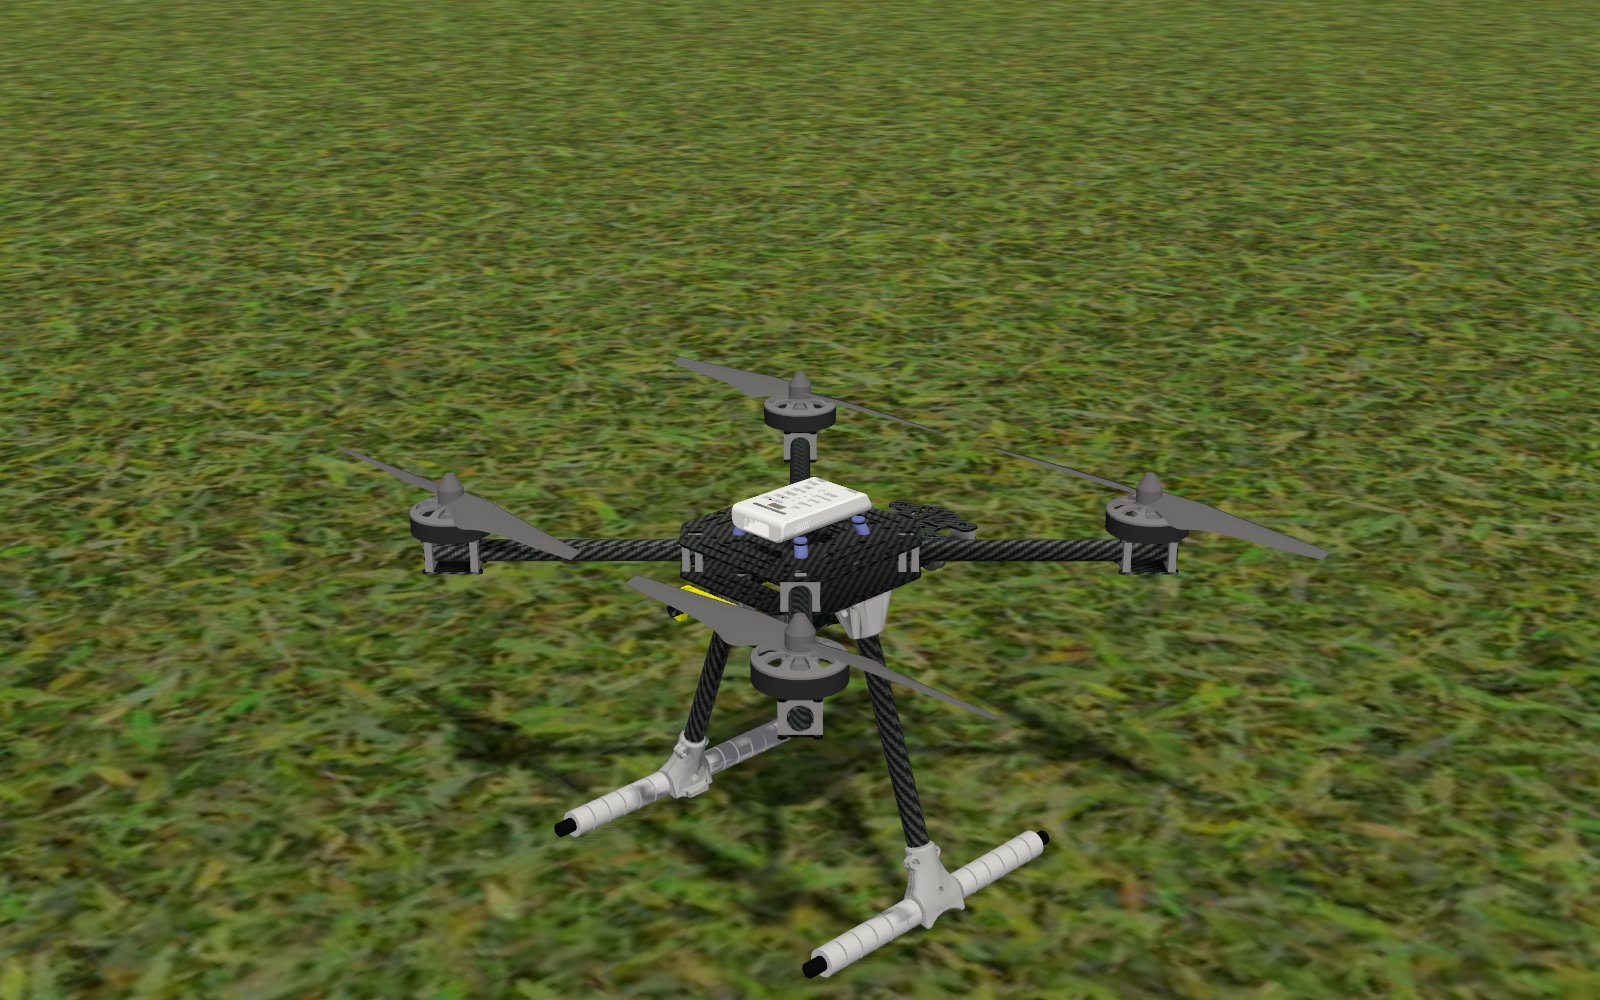
\includegraphics[width=\linewidth]{x500_tres_cuartos}
  \end{columns}
\end{frame}

\begin{frame}[fragile]{Paso 2: escuchar}
  \begin{lstlisting}[style=bash]
ros2 run px4_examples telemetry_listener     # en otra terminal
ros2 run px4_examples flight_mode_monitor    # en otra más
  \end{lstlisting}
  \small Déjenlos corriendo: les van a contar todo lo que pase en los siguientes pasos.
  \begin{idea}
    \small Si \cmd{telemetry\_listener} no recibe nada, \textbf{no sigan}: primero hay que arreglar la
    conexión (¿corre el agente?, ¿corre PX4?).
  \end{idea}
\end{frame}

\begin{frame}[fragile]{Paso 3: despegar}
  \begin{lstlisting}[style=bash]
ros2 run px4_examples takeoff_mission
  \end{lstlisting}
  \begin{columns}[c]
    \column{0.5\textwidth}\small
    Lo que debería pasar:
    \begin{enumerate}
      \item En \cmd{flight\_mode\_monitor}: \textbf{ARMADO} y \textbf{Hold $\rightarrow$ Offboard}.
      \item En QGC el modo dice Offboard y la altura sube.
      \item En Gazebo el dron se eleva y se queda a 5 m.
    \end{enumerate}
    \column{0.47\textwidth}\centering
    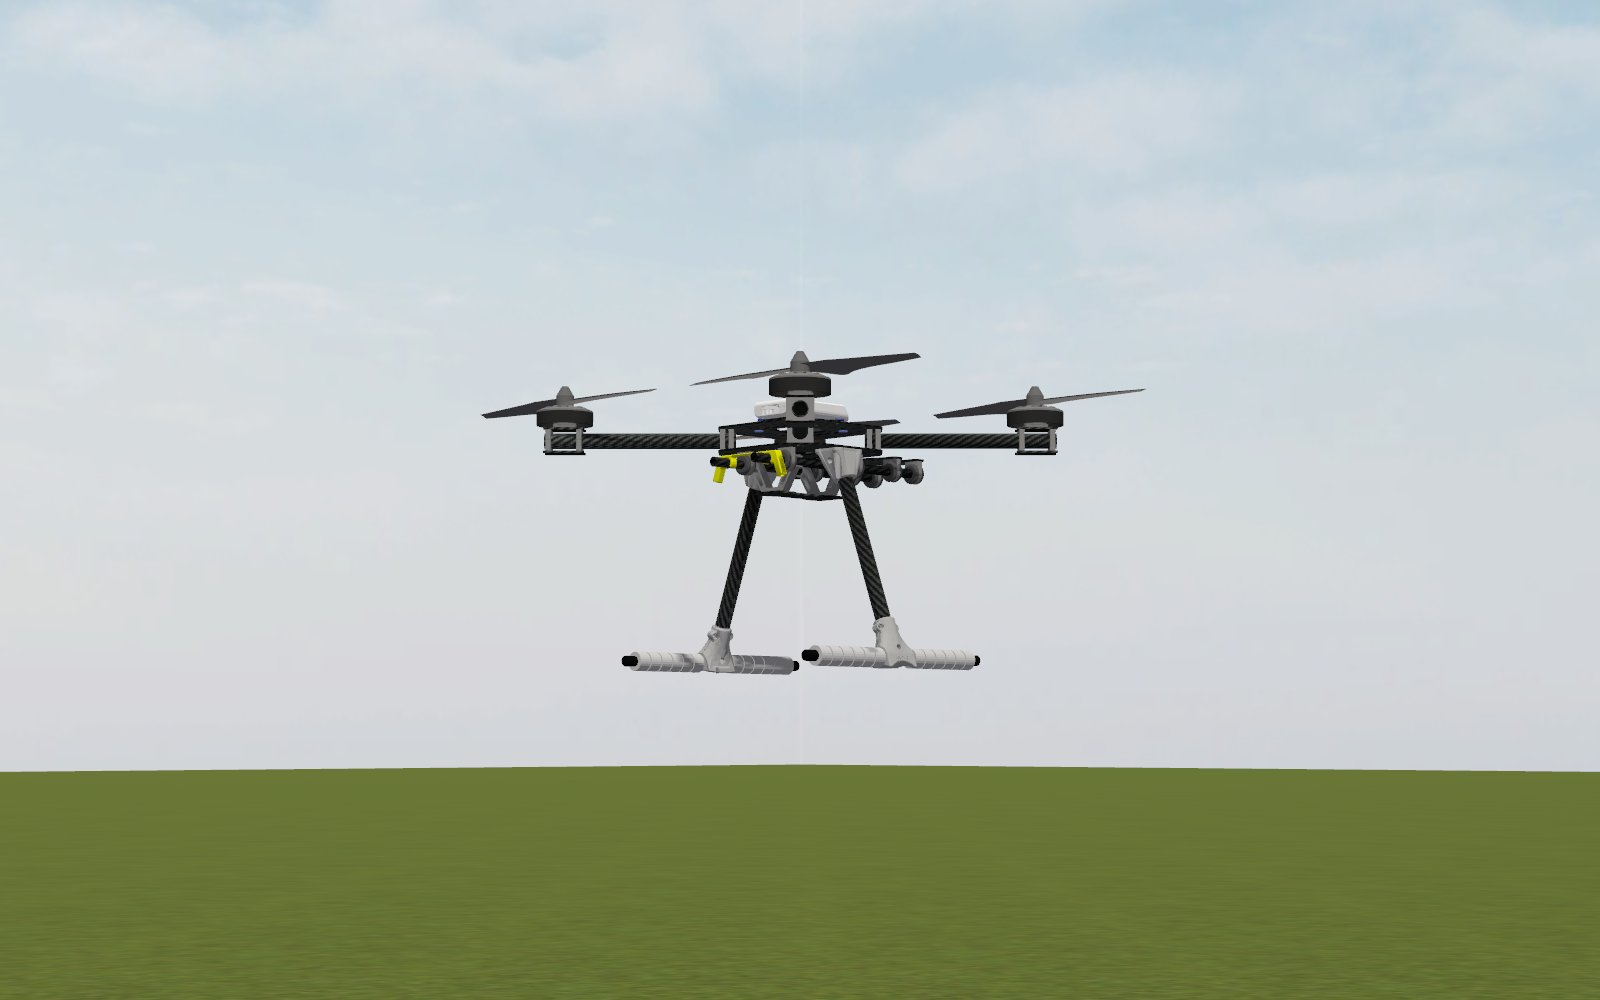
\includegraphics[width=\linewidth]{x500_volando}
  \end{columns}
\end{frame}

\begin{frame}{Paso 4: romperlo a propósito}
  \begin{columns}[c]
    \column{0.55\textwidth}\small
    Con el dron arriba, den \textbf{Ctrl+C} en \cmd{takeoff\_mission}:
    \begin{itemize}
      \item El nodo deja de publicar setpoints.
      \item En \textasciitilde0.5 s PX4 se da cuenta y entra en \textbf{failsafe}.
      \item Lo verán en \cmd{flight\_mode\_monitor} y en QGC.
    \end{itemize}
    Después aterricen con el botón \textbf{Land} de QGC.
    \column{0.42\textwidth}
    \begin{idea}
      \small Así se aprende que tu nodo \textbf{no está solo}: PX4 siempre está vigilando, y cuando algo
      falla toma el control.
    \end{idea}
  \end{columns}
\end{frame}

\begin{frame}{Y después}
  \begin{columns}[c]
    \column{0.5\textwidth}\small
    \textbf{Parte 2: PX4 + ROS 2 con px4\_examples}
    \begin{itemize}
      \item Instalar todo con \cmd{vespo}, paso a paso.
      \item Escuchar al dron y volarlo: \cmd{square\_mission} cuadro por cuadro.
      \item \cmd{shared\_ptr}, comandos de PX4 y tu primer reto: la estrella.
    \end{itemize}
    \vspace{0.3em}
    \textbf{Luego: las misiones de x500\_retos}, cada una en su propio mundo.
    \column{0.47\textwidth}\centering
    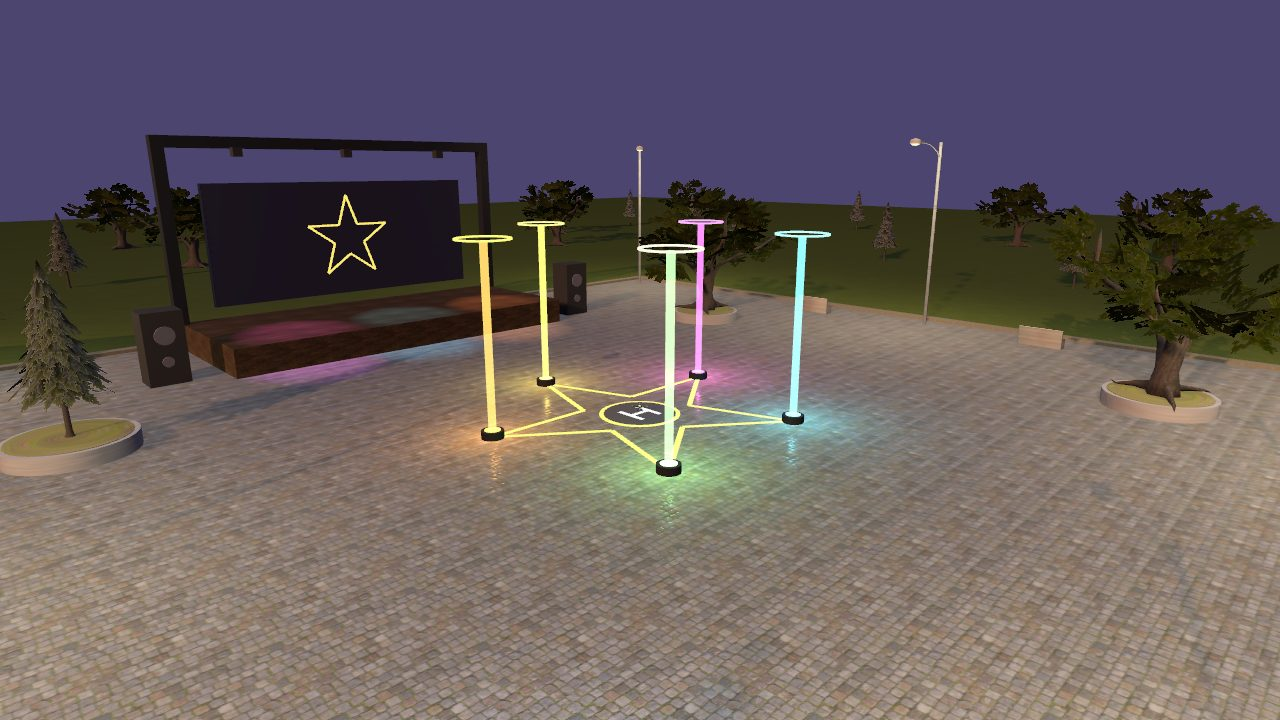
\includegraphics[width=\linewidth]{plaza_show_estrella}\\
    \credito{plaza\_show, de x500\_retos (render propio)}
  \end{columns}
\end{frame}

\begin{frame}{Créditos de las imágenes}
  \small
  \begin{itemize}
    \item \textbf{Fotos del X500, la Pixhawk 6C, el GPS M9N, la radio de telemetría, QGroundControl, Gazebo y el
      diagrama de uXRCE-DDS}: documentación de PX4 (\cmd{docs.px4.io}), © PX4 / Dronecode y colaboradores,
      licencia \textbf{CC BY 4.0} (\cmd{creativecommons.org/licenses/by/4.0}). Solo se redimensionaron.
    \item \textbf{Renders del x500 y de los mundos}: propios, hechos con Gazebo Harmonic sobre el modelo
      \cmd{x500} de PX4 (\cmd{tools/renders\_x500.py}).
  \end{itemize}
  \vspace{0.6em}
  \centering
\includegraphics[height=1.4cm]{vespo_logo}
\end{frame}

\end{document}
